% Options for packages loaded elsewhere
\PassOptionsToPackage{unicode}{hyperref}
\PassOptionsToPackage{hyphens}{url}
\PassOptionsToPackage{dvipsnames,svgnames,x11names}{xcolor}
\documentclass[
  11pt,
  letterpaper,
]{article}
\usepackage{xcolor}
\usepackage[margin=1in]{geometry}
\usepackage{amsmath,amssymb}
\setcounter{secnumdepth}{-\maxdimen} % remove section numbering
\usepackage{iftex}
\ifPDFTeX
  \usepackage[T1]{fontenc}
  \usepackage[utf8]{inputenc}
  \usepackage{textcomp} % provide euro and other symbols
\else % if luatex or xetex
  \usepackage{unicode-math} % this also loads fontspec
  \defaultfontfeatures{Scale=MatchLowercase}
  \defaultfontfeatures[\rmfamily]{Ligatures=TeX,Scale=1}
\fi
\usepackage{lmodern}
\ifPDFTeX\else
  % xetex/luatex font selection
\fi
% Use upquote if available, for straight quotes in verbatim environments
\IfFileExists{upquote.sty}{\usepackage{upquote}}{}
\IfFileExists{microtype.sty}{% use microtype if available
  \usepackage[]{microtype}
  \UseMicrotypeSet[protrusion]{basicmath} % disable protrusion for tt fonts
}{}
\usepackage{setspace}
\makeatletter
\@ifundefined{KOMAClassName}{% if non-KOMA class
  \IfFileExists{parskip.sty}{%
    \usepackage{parskip}
  }{% else
    \setlength{\parindent}{0pt}
    \setlength{\parskip}{6pt plus 2pt minus 1pt}}
}{% if KOMA class
  \KOMAoptions{parskip=half}}
\makeatother
\usepackage{longtable,booktabs,array}
\newcounter{none} % for unnumbered tables
\usepackage{calc} % for calculating minipage widths
% Correct order of tables after \paragraph or \subparagraph
\usepackage{etoolbox}
\makeatletter
\patchcmd\longtable{\par}{\if@noskipsec\mbox{}\fi\par}{}{}
\makeatother
% Allow footnotes in longtable head/foot
\IfFileExists{footnotehyper.sty}{\usepackage{footnotehyper}}{\usepackage{footnote}}
\makesavenoteenv{longtable}
\usepackage{graphicx}
\makeatletter
\newsavebox\pandoc@box
\newcommand*\pandocbounded[1]{% scales image to fit in text height/width
  \sbox\pandoc@box{#1}%
  \Gscale@div\@tempa{\textheight}{\dimexpr\ht\pandoc@box+\dp\pandoc@box\relax}%
  \Gscale@div\@tempb{\linewidth}{\wd\pandoc@box}%
  \ifdim\@tempb\p@<\@tempa\p@\let\@tempa\@tempb\fi% select the smaller of both
  \ifdim\@tempa\p@<\p@\scalebox{\@tempa}{\usebox\pandoc@box}%
  \else\usebox{\pandoc@box}%
  \fi%
}
% Set default figure placement to htbp
\def\fps@figure{htbp}
\makeatother
\setlength{\emergencystretch}{3em} % prevent overfull lines
\providecommand{\tightlist}{%
  \setlength{\itemsep}{0pt}\setlength{\parskip}{0pt}}
% Layout additions for manuscript.tex and supplement.tex (pandoc inlines this file into each preamble).
\usepackage{url}                 % \path for file names, commits and hashes (breakable; see code_path.lua)
\usepackage{caption}
\captionsetup{font=small,labelformat=empty,justification=justified,singlelinecheck=false,list=no,skip=6pt}
\usepackage[section]{placeins}   % figures do not float past the end of their section
\usepackage{etoolbox}
\AtBeginEnvironment{longtable}{\small}
\setlength{\LTpre}{8pt}
\setlength{\LTpost}{8pt}
\raggedbottom
\setlength{\parskip}{3pt plus 1pt}
\makeatletter
\renewcommand{\@seccntformat}[1]{\csname the#1\endcsname\quad}
\def\fps@figure{!htbp}
\renewcommand{\topfraction}{0.9}
\renewcommand{\bottomfraction}{0.8}
\renewcommand{\textfraction}{0.07}
\renewcommand{\floatpagefraction}{0.8}
\makeatother
\ifPDFTeX
  % pdfLaTeX (for example on arXiv): every non-ASCII character of manuscript.tex and supplement.tex, which XeTeX takes
  % from the font. build.sh lists the non-ASCII characters of both files and stops if one is not declared here.
  \DeclareUnicodeCharacter{2212}{\ensuremath{-}}        % minus sign
  \DeclareUnicodeCharacter{00B1}{\ensuremath{\pm}}      % plus-minus sign
  \DeclareUnicodeCharacter{2265}{\ensuremath{\geq}}     % greater-than or equal to
  \DeclareUnicodeCharacter{2264}{\ensuremath{\leq}}     % less-than or equal to
  \DeclareUnicodeCharacter{00D7}{\ensuremath{\times}}   % multiplication sign
  \DeclareUnicodeCharacter{00B5}{\ensuremath{\mu}}      % micro sign
  \DeclareUnicodeCharacter{00FC}{\"{u}}                 % u with diaeresis (a reference author's name)
  \DeclareUnicodeCharacter{00E9}{\'{e}}                 % e with acute (a reference author's name)
  \DeclareUnicodeCharacter{00E1}{\'{a}}                 % a with acute (a reference author's name)
  \DeclareUnicodeCharacter{2081}{\ensuremath{_1}}
  \DeclareUnicodeCharacter{2082}{\ensuremath{_2}}
\fi
% The author line is long: set it in a centred paragraph that can wrap, not in the default unbreakable tabular.
\usepackage{titling}
\pretitle{\begin{center}\LARGE\bfseries}
\posttitle{\par\end{center}\vskip 0.4em}
\preauthor{\begin{center}\large\begin{minipage}{0.92\textwidth}\centering}
\postauthor{\end{minipage}\par\end{center}}
\predate{\begin{center}\normalsize}
\postdate{\par\end{center}}
% Table captions sit at the top of their longtable (table_captions.lua) and span the text width.
\setlength{\LTcapwidth}{\textwidth}
\usepackage{bookmark}
\IfFileExists{xurl.sty}{\usepackage{xurl}}{} % add URL line breaks if available
\urlstyle{same}
% fallback for those not using the hyperref driver hyperxmp:
\makeatletter
\@ifundefined{xmpquote}{\newcommand{\xmpquote}[1]{#1}}{}
\makeatother
\hypersetup{
  pdftitle={Supplementary Information},
  pdfauthor={Mateenah Jahan and Marouen Ben Guebila},
  colorlinks=true,
  linkcolor={Maroon},
  filecolor={Maroon},
  citecolor={Blue},
  urlcolor={Blue},
  pdfcreator={LaTeX via pandoc}}

\title{Supplementary Information}
\usepackage{etoolbox}
\makeatletter
\providecommand{\subtitle}[1]{% add subtitle to \maketitle
  \apptocmd{\@title}{\par {\large #1 \par}}{}{}
}
\makeatother
\subtitle{Sex-chromosome expression and annotated donor sex in
drug-perturbation cell lines}
\author{Mateenah Jahan and Marouen Ben Guebila}
\date{}

\begin{document}
\maketitle

\setstretch{1.12}
\section*{Contents}\label{contents}
\addcontentsline{toc}{section}{Contents}

\begin{itemize}
\tightlist
\item
  Glossary
\item
  Table S1. Expression-state table and column definitions
\item
  Note S1. Data sources and external states (Table S2)
\item
  Note S2. Vehicle cells
\item
  Note S3. State calling (Table S3)
\item
  Note S4. Agreement between the Tahoe-100M implementations
\item
  Note S5. Expression-state checks and subpopulation criteria (Table S4)
\item
  Note S6. Depth matching across cultures
\item
  Note S7. EmeraldBay and sci-Plex calls
\item
  Note S8. Timing of analyses and interpretation (Table S5)
\item
  Note S9. Per-line notes (Table S6)
\item
  Note S10. Donor labels and agreement across cultures
\item
  Note S11. Ambient RNA and marker-rich cells (Figure S1)
\item
  Note S12. Marker-negative cells (Table S7, Figure S2)
\item
  Note S13. Depth-matched comparison results (Table S8)
\item
  Note S14. STR Amelogenin comparison
\item
  Note S15. Data and code availability
\item
  Note S16. Part B design (Tables S9 to S11)
\item
  Note S17. Part B results, sensitivity and power (Tables S12 and S13,
  Figure S3)
\item
  Note S18. Part B exploratory follow-ups (Table S14)
\item
  Note S19. Earlier analyses of overlapping data
\end{itemize}

References are listed in the manuscript.

\section{Glossary}\label{glossary}

{\def\LTcaptype{none} % do not increment counter
\begin{longtable}[]{@{}
  >{\raggedright\arraybackslash}p{(\linewidth - 2\tabcolsep) * \real{0.4000}}
  >{\raggedright\arraybackslash}p{(\linewidth - 2\tabcolsep) * \real{0.6000}}@{}}
\toprule\noalign{}
\begin{minipage}[b]{\linewidth}\raggedright
Term
\end{minipage} & \begin{minipage}[b]{\linewidth}\raggedright
Meaning
\end{minipage} \\
\midrule\noalign{}
\endhead
\bottomrule\noalign{}
\endlastfoot
P1 & Primary LINCS2020 panel, ASG project (1.0 µM, 24 h) \\
P1b & Lower-dose panel from the ASG project (0.1 µM, 24 h) \\
P2 & Second panel, CPC project (10 µM, 6 h) \\
Level 3 & Well-level expression after subtracting the mean of the same
plate's DMSO wells, per gene \\
Level 5 & CMap consensus z-scores scaled against the wells of each
plate \\
H1 to H4 & Panel-level test, per-compound tests, pooled response-size
difference and annotated-sex comparison, respectively \\
T\textsubscript{c} & Mean squared t statistic across 978 landmark genes
for one compound and model term \\
s & Response size for one line and compound, relative to the mean
response of the other lines \\
S & A line's mean response size across compounds \\
E1 to E5 & Gene-level effect in residual SD units, compound-level
response-size difference, pooled response-size difference, count of
nominal per-compound results, and excess of the observed panel statistic
over its null median, respectively \\
\end{longtable}
}

\section{Part A: measured states}\label{part-a-measured-states}

\subsection{Table S1. Expression-state table and column
definitions}\label{table-s1.-expression-state-table-and-column-definitions}

The separate file \path{supplementary_table_S1.tsv} contains 1,694 rows
for 1,123 cell lines. Each row is identified by its Cellosaurus
accession and data source. Vehicle-cell rows come from Tahoe-100M (50),
EmeraldBay (52) and sci-Plex (6). The remaining rows cover LINCS2020
(139), GDSC2 (969) and PRISM (478). These contain states derived from
bulk RNA-seq when available. 21 rows lack RNA-seq and are marked
\path{not_measured}. Lines screened in both GDSC2 and PRISM have one row
for each screen. NCI-H1975 appears under two CMap names, so the 140
LINCS2020 names with RNA-seq contribute 139 rows.

LINCS2020 rows use Cellosaurus donor annotations. The analysis used
CMap's label when available. Some rows therefore have a state in Table
S1 that was ambiguous in the original analysis because the CMap label
was missing. The table contains derived expression states from CCLE and
Cell Model Passports RNA-seq and excludes the original input
measurements and CMap's annotation file. Treat sci-Plex calls as
qualitative (Note S3). Interpret the four Tahoe-100M single-arm
expression patterns with the filter caveat in Note S9. NCI-H596's
Tahoe-100M call is low confidence and should be treated as uncertain.
The existing file uses the state codes defined in Table S3. An empty
cell indicates an unavailable or inapplicable field.

{\def\LTcaptype{none} % do not increment counter
\begin{longtable}[]{@{}
  >{\raggedright\arraybackslash}p{(\linewidth - 2\tabcolsep) * \real{0.4706}}
  >{\raggedright\arraybackslash}p{(\linewidth - 2\tabcolsep) * \real{0.5294}}@{}}
\toprule\noalign{}
\begin{minipage}[b]{\linewidth}\raggedright
Column
\end{minipage} & \begin{minipage}[b]{\linewidth}\raggedright
Content
\end{minipage} \\
\midrule\noalign{}
\endhead
\bottomrule\noalign{}
\endlastfoot
\path{cellosaurus_id} & Cellosaurus accession \\
\path{source} & Tahoe-100M, EmeraldBay, sciPlex2, sciPlex3 or sciPlex4
for vehicle cells. LINCS2020, GDSC2 or PRISM for lines assessed by bulk
RNA-seq \\
\path{cell_name} & Line name in the data source \\
\path{called_by} & Analysis that supplied the call \\
\path{line_id} & Line identifier in GDSC2 or PRISM \\
\path{cmp_model_id} & Cell Model Passports identifier where available \\
\path{organ} & Organ of origin in vehicle-cell dataset metadata \\
\path{sex_label} & Donor-sex annotation used in the rule. For GDSC2 and
PRISM, disagreement between Cellosaurus and Cell Model Passports is
coded \path{conflict} \\
\path{state} & Label-relative expression code (Table S3), or
\path{not_measured} \\
\path{confidence} & High, medium or low for vehicle-cell calls \\
\path{arm_state} & Expression pattern of the Yp and Yq marker sets.
Legacy codes \texttt{Y\ intact}, \texttt{Yq\ lost}, \texttt{Yp\ lost}
and \texttt{Y\ lost} mean both scores high, Yp alone high, Yq alone high
and both scores low, respectively \\
\path{n_vehicle_cells} & Number of vehicle cells in the line \\
\path{n_vehicle_cells_called} & Tahoe-100M cells remaining after the
marker-rich filter \\
\path{n_units} & Vehicle-cell batches with sufficient cells. Units are
Tahoe-100M plates, EmeraldBay samples, sci-Plex culture plates or the
pooled line \\
\path{units_agree} & Number of batch pseudobulks whose calls agree with
the line-level call \\
\path{grid_stable} & Whether the call holds across all shifts of the
expression cut-offs \\
\path{xist} & Vehicle-cell XIST expression in log2(CPM+1) \\
\path{y_score} & Mean of the Y-marker scores on that scale \\
\path{yp_score} & Mean of the Yp-marker scores on that scale \\
\path{yq_score} & Mean of the Yq-marker scores on that scale \\
\path{mosaic_marker} & Y or XIST in A549, SW48 and the two negative
controls \\
\path{mosaic_verdict} & Subpopulation criterion outcome for those four
lines \\
\path{negative_share_lo} & Lowest output across estimators and
implementations (Note S12) \\
\path{negative_share_hi} & Highest output across estimators and
implementations (Note S12) \\
\end{longtable}
}

\subsection{Note S1. Data sources and external
states}\label{note-s1.-data-sources-and-external-states}

We accessed the initial inputs on 14 November 2026 and 15 November 2026,
and the Cellosaurus STR records on 16 November 2026.

\begin{longtable}[]{@{}
  >{\raggedright\arraybackslash}p{(\linewidth - 6\tabcolsep) * \real{0.0741}}
  >{\raggedright\arraybackslash}p{(\linewidth - 6\tabcolsep) * \real{0.4815}}
  >{\raggedright\arraybackslash}p{(\linewidth - 6\tabcolsep) * \real{0.2222}}
  >{\raggedright\arraybackslash}p{(\linewidth - 6\tabcolsep) * \real{0.2222}}@{}}
\caption{\textbf{Table S2. Data sources.}}\tabularnewline
\toprule\noalign{}
\begin{minipage}[b]{\linewidth}\raggedright
ID
\end{minipage} & \begin{minipage}[b]{\linewidth}\raggedright
Source
\end{minipage} & \begin{minipage}[b]{\linewidth}\raggedright
Used for
\end{minipage} & \begin{minipage}[b]{\linewidth}\raggedright
Licence or access
\end{minipage} \\
\midrule\noalign{}
\endfirsthead
\toprule\noalign{}
\begin{minipage}[b]{\linewidth}\raggedright
ID
\end{minipage} & \begin{minipage}[b]{\linewidth}\raggedright
Source
\end{minipage} & \begin{minipage}[b]{\linewidth}\raggedright
Used for
\end{minipage} & \begin{minipage}[b]{\linewidth}\raggedright
Licence or access
\end{minipage} \\
\midrule\noalign{}
\endhead
\bottomrule\noalign{}
\endlastfoot
D1 & Tahoe-100M (Zhang et al.~2026): Hugging Face dataset
\path{tahoebio/Tahoe-100M}, revision
\path{349e2a55f5538a3e73b32a06c6bdd8e9e87011e8}; raw counts and cell,
sample, line and gene metadata & vehicle cells of 50 lines & CC0 \\
D2 & EmeraldBay: Hugging Face dataset \path{tahoebio/EmeraldBay} &
vehicle cells of 52 lines & CC BY 4.0 \\
D3 & sci-Plex (Srivatsan et al.~2020): GEO series GSE139944, samples
GSM4150377 (sciPlex2), GSM4150378 (sciPlex3) and GSM4150379 (sciPlex4) &
vehicle cells of A549, MCF7 and K562 & GEO \\
D4 & CCLE legacy RNA-seq, gene RPKM (Ghandi et al.~2019):
\path{https://data.broadinstitute.org/ccle/CCLE_RNAseq_genes_rpkm_20180929.gct.gz}
& external expression states & public \\
D5 & Cell Model Passports RNA-seq and model list (van der Meer et
al.~2019):
\path{https://cog.sanger.ac.uk/cmp/download/rnaseq_latest.csv.gz},
\path{https://cog.sanger.ac.uk/cmp/download/model_list_20240110.csv} &
external states; line identifiers & public \\
D6 & Cellosaurus (Bairoch 2018), release 57.0:
\path{https://ftp.expasy.org/databases/cellosaurus/cellosaurus.txt} &
annotated sex (SX field) & public \\
D7 & CMap LINCS2020 cell annotation (Subramanian et al.~2017):
\path{https://s3.amazonaws.com/macchiato.clue.io/builds/LINCS2020/cellinfo_beta.txt}
& LINCS lines and CMap donor sex & public; LINCS files are not
redistributed \\
D8 & PIE context file:
\path{https://huggingface.co/datasets/arcinstitute/PIE_sources/resolve/main/context_text/descriptions.json}
& the ``Sex:'' field of each cell context & public \\
D9 & ATCC CCL-185 (A549) product page, karyotype section:
\path{https://www.atcc.org/products/ccl-185} & A549 seed-stock karyotype
& public \\
D10 & GDSC2 fitted dose response (Iorio et al.~2016) and PRISM secondary
screen (Corsello et al.~2020) & lists of screened lines only & public \\
D11 & Cellosaurus records by accession:
\path{https://api.cellosaurus.org/cell-line/<accession>?format=txt} &
STR Amelogenin results (DNA-level check, Note S14) & public \\
\end{longtable}

\textbf{External states.} The same density rule was applied separately
to the CCLE and Cell Model Passports RNA-seq datasets (Note S3). For
LINCS2020 lines, discordant RNA-seq calls were coded as ambiguous. For
GDSC2 and PRISM lines, Cell Model Passports was the primary source and
CCLE was used where that source lacked data. The latter analysis used
the consensus donor label from Cell Model Passports and Cellosaurus,
with disagreement coded as a conflict.

External RNA-seq was available for 140 of 240 LINCS2020 lines, including
135 in CCLE. Calls agreed across both sources for 17 of 18 with both
measurements. HCT116 differed and was coded ambiguous. The two RNA-seq
sources agreed for 729 of 755 lines covered by both GDSC2/PRISM
reference datasets. Inferred L1000 Y scores had a Spearman correlation
of 0.21 with CCLE scores over 124 lines and yielded AUC 0.53 for
separating Y-high and Y-low lines.

\subsection{Note S2. Vehicle cells}\label{note-s2.-vehicle-cells}

\textbf{Tahoe-100M.} We selected cells with the \path{DMSO_TF} vehicle
annotation and \path{full} filter status in the atlas metadata (Zhang et
al.~2026). Vehicle wells were profiled at 24 h. Each of the 14 plates
contained 2 such wells with all 50 lines represented. Both
implementations matched the same 2,205,786 vehicle cells to the atlas
metadata by barcode, plate, sample and line, and verified UMI totals
against the metadata. Explicit zero entries contributed no UMIs.

Per cell we kept total UMIs, cell-cycle phase (from \path{obs_metadata})
and the counts of XIST and TSIX; the 8 Y genes RPS4Y1, DDX3Y, KDM5D,
UTY, EIF1AY, ZFY, USP9Y and NLGN4Y; TXLNGY and PRKY (secondary); their X
gametologs RPS4X, DDX3X, KDM5C, KDM6A, EIF1AX, ZFX, USP9X and NLGN4X;
and ACTB and GAPDH. Per line and well we kept all-gene pseudobulk
counts.

\textbf{EmeraldBay.} Vehicle cells are those with drug ``DMSO\_TF'':
100,253 cells of 52 lines, out of 1,831,648 cells in all. EmeraldBay has
no plate field, so its 4 vehicle samples are the batch unit. The dataset
provides no quality filter, so no cell was removed. Time-zero controls
(``DMSO\_T0'') were left out. Depth is the sum of counts over gene
tokens.

\textbf{sci-Plex.} Vehicle cells came from the authors' labels in
sciPlex3, and from vehicle hashes with fixed hash-quality filters in
sciPlex2 and sciPlex4. This gave 2,631 vehicle cells in sciPlex2 (A549
only), 17,578 in sciPlex3 (A549, MCF7 and K562) and 3,361 in sciPlex4
(A549 and MCF7). Depth counts human genes only. sci-Plex labels and
sequences nuclei (``nuclear hashing''; Srivatsan et al.~2020), so its
counts come from nuclear RNA, in which XIST is enriched.

No treated cell enters any state call, cut-off, background or mosaic
estimate. The second-culture identity check pooled deep cells across
treated and vehicle conditions without using their condition labels.

\subsection{Note S3. State calling}\label{note-s3.-state-calling}

Scores. For a set of cells, the CPM of a gene is its summed UMIs per
million summed UMIs. XIST is log2(CPM+1). The Y score is the mean
log2(CPM+1) of the 8 Y genes. The Yp score uses RPS4Y1 and ZFY, and the
Yq score uses DDX3Y, USP9Y, UTY, NLGN4Y, KDM5D and EIF1AY. Small
pseudobulks can yield lower average log expression because more genes
have zero observed UMIs.

Units. In Tahoe-100M the primary unit is one line on one plate, the sum
of the plate's vehicle wells (700 units). The line state comes from the
line's pseudobulk over all plates, so cut-offs fitted on plate units are
applied to line pseudobulks. EmeraldBay uses one line in one vehicle
sample, and sci-Plex one line on one culture plate; sciPlex2 has no
batch unit.

\textbf{Cut-offs.} A Gaussian kernel density
(\path{scipy.stats.gaussian_kde}, Scott bandwidth) is evaluated on 1,024
points from the lowest to the highest value, and the cut-off is the
point of lowest density between the two tallest modes. No interval is
given for a cut-off; the grid of shifted cut-offs below shows which
calls depend on its exact place. In Tahoe-100M the primary cut-offs come
from the line-by-plate values; line-level cut-offs, from one value per
line, are a sensitivity analysis. EmeraldBay used its own line-by-sample
values, from units with at least 10 vehicle cells. sci-Plex has too few
lines for a density, so we applied the bulk CCLE cut-offs (XIST 1.98 and
Y score 1.31, in log2(RPKM+1)) on single-cell pseudobulk CPM, with the Y
cut-off for both arms, and repeated the calls with EmeraldBay's
cut-offs. The units and the cell compartment differ (whole-cell bulk
RPKM against nuclear CPM), so the sci-Plex calls are qualitative;
EmeraldBay's cut-offs gave the same calls.

Patterns and states. A score at or above its cut-off is high. The two
scores give each line a label-independent pattern: Y only (Y high, XIST
low), XIST only (XIST high, Y low), both, or neither. Table S3 gives the
donor-label-relative codes used in the existing data file. A missing
value gives ``ambiguous''.

\begin{longtable}[]{@{}lllll@{}}
\caption{\textbf{Table S3. Rule table.}}\tabularnewline
\toprule\noalign{}
Y score & XIST & Label Female & Label Male & No label \\
\midrule\noalign{}
\endfirsthead
\toprule\noalign{}
Y score & XIST & Label Female & Label Male & No label \\
\midrule\noalign{}
\endhead
\bottomrule\noalign{}
\endlastfoot
high & any & discordant & XY & XY \\
low & high & XX-like & discordant & XX-like \\
low & low & XIST-lost & Y-lost & ambiguous \\
\end{longtable}

The codes describe thresholded expression. For example, both
\path{Y-lost} and \path{XIST-lost} encode scores below both cut-offs,
with the choice of code depending on the recorded donor label.
\path{XX-like} encodes XIST-high and Y-low expression. Chromosome copy
number and X inactivation require separate evidence.

\textbf{Labels and cell counts.} We used the Cellosaurus donor
annotation when available. Both the Cellosaurus and PIE records identify
hTERT-HPNE as male. RKO had no recorded annotation in the records used.
The EmeraldBay analysis used Cellosaurus annotations, supplemented with
PIE when needed. The 200-cell minimum after marker-rich filtering
applies to Tahoe-100M. In EmeraldBay, the 10-cell threshold screened
sample-level pseudobulks for estimation of the cut-offs. Pooled lines
could still receive a low-confidence call when all their samples fell
below that threshold (Note S10).

Confidence. Each plate's pseudobulk is called with the same cut-offs as
the line. A call has high confidence if every plate gives the line's
call and the line's call is unchanged when each cut-off is kept or moved
by 1 log2 unit up or down (9 combinations). It has medium confidence if
it is not high and at least 80\% of plates agree, and low confidence
otherwise. In EmeraldBay, with 4 vehicle samples, medium can only mean
that every sample agrees but the call is not stable on the grid. For
sciPlex2, which has no batch unit, confidence uses the grid only.

\textbf{Arm patterns.} The same density rule sets the cut-offs for Yp
and Yq in Tahoe-100M (line-by-plate values) and EmeraldBay
(line-by-sample values). sci-Plex uses the bulk CCLE Y cut-off for both
scores. For male-labelled lines, we report whether both, neither, or
just one of the two marker sets exceeds its cut-off.

Marker-rich filter. Pooled wells carry ambient RNA, and some cells are
doublets or are assigned to the wrong line. Before calling, each
pipeline removed marker-rich cells. In a line whose Y score was below
the cut-off, it removed cells with 3 or more UMIs summed over the 8 Y
genes. In a line whose XIST was below the cut-off, it removed cells with
3 or more XIST UMIs. A line is never filtered on its own high marker.
The local caller set each line's status from all cells, then refiltered
and recomputed the cut-offs until the status no longer changed (2
rounds). The cloud implementation set status from all cells, removed
marker-rich cells, then estimated final cut-offs and calls. Both report
the calls made before removal, which equal the final calls. The filter
selects on the marker itself: in lines that express part of the Y marker
set, many removed cells are the line's own (Note S9), and in a small
line whose score is lifted by marker-rich cells, the filter is not
applied at all (NCI-H596, Note S9).

\subsection{Note S4. Agreement between the Tahoe-100M
implementations}\label{note-s4.-agreement-between-the-tahoe-100m-implementations}

Two implementations applied the same calling rules to the same
Tahoe-100M cells. The resulting tables were joined by Cellosaurus
accession and compared for state, confidence, Y-arm expression pattern,
plate agreement, grid stability, cell counts and scores. Agreement tests
implementation consistency. External RNA-seq and STR Amelogenin
comparisons provide separate evidence about the calls (Notes S9 and
S14).

The agreement criterion required matching calls for at least 48 of 50
lines. Where the methods allowed different choices, the implementations
differed in four ways.

\begin{itemize}
\tightlist
\item
  The local implementation excluded selected partial-Y lines from its Y
  background estimate, while the cloud implementation used all Y-low
  lines.
\item
  For the identity comparison in criterion (f), the local implementation
  depth-matched the comparison line and used autosomal and X-linked
  genes above 10 CPM. The cloud implementation used full pseudobulk
  profiles and included genes above 1 CPM after excluding the Y markers,
  XIST, TSIX, mitochondrial and TTTY genes.
\item
  The local implementation reapplied the marker-rich filter for the
  line-level sensitivity analysis. The cloud implementation retained the
  primary filter.
\item
  The local implementation used filtered vehicle cells for the
  subpopulation tests. The cloud implementation used all vehicle cells.
\end{itemize}

The marker-rich filter excluded cells from 46 lines and left 2,175,916
cells. Every line retained at least 200 cells, and 48 retained at least
1,000.

Each score had exactly two modes at both levels. The primary cut-offs,
in log2(CPM+1), were XIST 4.68 (modes 1.54 and 8.18), Y score 4.02
(modes 1.49 and 5.68), Yp 3.96 and Yq 3.58, the same in both pipelines.
In the local implementation, a wider density grid moved no cut-off by
more than 0.008 log2 units.

The pipelines agreed on state and confidence for 50 of 50 lines and on
arm state for 50. They also agreed on every line's plate agreement, grid
stability and cell counts, and their scores differed by at most 0.00005
log2 units, the rounding of the local table.

Under line-level cut-offs, a sensitivity analysis, the pipelines gave
the same state for 48 of 50 lines. Their line-level cut-offs differed
(local: XIST 5.527 and Y 3.742; the cloud implementation: 5.534 and
3.789) because the local implementation redid the filter under these
cut-offs and the cloud implementation did not. In the local
implementation, COLO 205 became XY: it counted as Y-positive and kept
its 3,052 cells with 3 or more Y UMIs. NCI-H2122 became discordant. the
cloud implementation's line-level calls changed no line. The label-audit
count was the same under line-level cut-offs in both pipelines, although
in the local implementation COLO 205 left the list and NCI-H2122 joined
it.

\subsection{Note S5. Expression-state checks and subpopulation
criteria}\label{note-s5.-expression-state-checks-and-subpopulation-criteria}

\begin{longtable}[]{@{}
  >{\raggedright\arraybackslash}p{(\linewidth - 4\tabcolsep) * \real{0.2000}}
  >{\raggedright\arraybackslash}p{(\linewidth - 4\tabcolsep) * \real{0.5714}}
  >{\raggedright\arraybackslash}p{(\linewidth - 4\tabcolsep) * \real{0.2286}}@{}}
\caption{\textbf{Table S4. Expression-state checks and
interpretation.}}\tabularnewline
\toprule\noalign{}
\begin{minipage}[b]{\linewidth}\raggedright
Check
\end{minipage} & \begin{minipage}[b]{\linewidth}\raggedright
Rule or comparison
\end{minipage} & \begin{minipage}[b]{\linewidth}\raggedright
Timing
\end{minipage} \\
\midrule\noalign{}
\endfirsthead
\toprule\noalign{}
\begin{minipage}[b]{\linewidth}\raggedright
Check
\end{minipage} & \begin{minipage}[b]{\linewidth}\raggedright
Rule or comparison
\end{minipage} & \begin{minipage}[b]{\linewidth}\raggedright
Timing
\end{minipage} \\
\midrule\noalign{}
\endhead
\bottomrule\noalign{}
\endlastfoot
Agreement with external RNA-seq (A1) & At least 90\% agreement among
comparable lines. Agreement below 80\% would suggest that state calls
depend strongly on culture & Specified before the full Tahoe-100M
calls \\
Agreement with EmeraldBay (A2) & At least 90\% agreement among shared
lines with medium or high confidence in both atlases & Exploratory.
Preliminary results from the other cultures were already available \\
Depth matching (A3) & Absolute difference of at most 0.15 for the usable
estimators in A549 and SW48 & Exploratory. The detailed procedure
preceded the matched estimates (Note S8) \\
Donor-label audit (A4) & Count mismatches under each set of cut-offs &
Specified before the full Tahoe-100M calls \\
Y-arm expression (A5) & Compare Yp and Yq scores for each male-labelled
line & Specified before the full Tahoe-100M calls \\
Ambient RNA and marker-rich cells (A6) & Estimate plate background and
marker-rich cell shares & Specified before the full Tahoe-100M calls \\
Plate consistency & Count line-by-plate calls matching the line-level
call & Post hoc \\
Negative controls & NCI-H460 and LoVo should fail the subpopulation
rule. Y-arm zero co-occurrence is compared with the X-gametolog control
& Specified before the full Tahoe-100M calls \\
\end{longtable}

\textbf{Subpopulation criteria.} We evaluated Y in Y-high lines and XIST
in XIST-high lines with at least 1,000 vehicle cells.

\begin{itemize}
\tightlist
\item
  \begin{enumerate}
  \def\labelenumi{(\alph{enumi})}
  \tightlist
  \item
    The share of cells with no marker UMI among cells with at least
    3,000 UMIs and among cells with at least 8,000 UMIs, with bootstrap
    95\% intervals, beside the share expected if every cell expressed
    the marker at the rate of the marker-positive cells.
  \end{enumerate}
\item
  \begin{enumerate}
  \def\labelenumi{(\alph{enumi})}
  \setcounter{enumi}{1}
  \tightlist
  \item
    A mixture model per cell: a low component at the plate's measured
    background rate, a negative-binomial high component, and a
    marker-negative share that is logistic in log depth, read at 1,000,
    2,000, 4,000 and 8,000 UMIs.
  \end{enumerate}
\item
  \begin{enumerate}
  \def\labelenumi{(\alph{enumi})}
  \setcounter{enumi}{2}
  \tightlist
  \item
    A two-component Poisson mixture with the plate background, as in the
    pilot and second-culture analysis.
  \end{enumerate}
\item
  \begin{enumerate}
  \def\labelenumi{(\alph{enumi})}
  \setcounter{enumi}{3}
  \tightlist
  \item
    Model (b) refitted on odd and on even plates.
  \end{enumerate}
\item
  \begin{enumerate}
  \def\labelenumi{(\alph{enumi})}
  \setcounter{enumi}{4}
  \tightlist
  \item
    For Y only: the Mantel-Haenszel odds ratio, over depth deciles, of
    ``no Yq UMI'' with ``no Yp UMI'', against the same odds ratio for
    two thinned halves of the X gametologs.
  \end{enumerate}
\item
  \begin{enumerate}
  \def\labelenumi{(\alph{enumi})}
  \setcounter{enumi}{5}
  \tightlist
  \item
    Identity: pooled deep (at least 2,500 UMIs) marker-negative cells
    compared with size- and depth-matched pools of the line's
    marker-positive cells, with a split-half of the positive cells, and
    with the most similar other line; and the nearest line centroid of
    single deep marker-negative cells.
  \end{enumerate}
\end{itemize}

A line is mosaic only if (b) at 2,000 UMIs lies between 0.15 and 0.85;
the odd-plate and even-plate fits in (d) differ by at most 0.10; the
odds ratio in (e) exceeds 2 times its control (Y only); and in (f) the
negative pool correlates with the positive pool within 0.01 of the
split-half and at least 0.10 above any other line. Shares are reported
as the span across (a) to (c), never as one number.

NCI-H460 and LoVo were selected as negative controls based on the pilot.
The study lacked a positive control with a known subpopulation. The
written rules did not specify how to resolve disagreement between the
implementations. After examining both results, we required both
implementations to meet the criteria before reporting a subpopulation.
The two candidate cases did not meet this requirement (Note S12).

\subsection{Note S6. Depth matching across
cultures}\label{note-s6.-depth-matching-across-cultures}

We compared marker-negative estimates for A549 and SW48 in Tahoe-100M,
EmeraldBay and sci-Plex. Because thinning only reduces UMI counts, we
thinned the deeper dataset in each pair. This meant thinning Tahoe-100M
for sciPlex3 and sciPlex4, which were shallower.

Pairs. The tests are A549 (Y) against EmeraldBay, sciPlex2, sciPlex3 and
sciPlex4, and SW48 (XIST) against EmeraldBay. NCI-H460 (Y) and LoVo (Y)
against EmeraldBay are context only, with no decision. They have no
known Y-negative subpopulation, so they show how far thinning and
culture alone move each estimator.

Thinning. The cells of the deeper dataset are ranked by depth, and each
cell's target depth is the shallower dataset's depth quantile at the
cell's mid-rank. If the target is below the cell's depth, each UMI is
kept independently with probability target over depth, for marker and
other UMIs alike. The shallower dataset and the per-UMI background are
not changed. There are 10 thinning replicates with fixed seeds. The
range over replicates reflects thinning only; it is not a confidence
interval and leaves out the sampling error of the cells.

Cells and backgrounds. Tahoe cells are the local implementation's
vehicle cells after its filter, with its per-plate background (Y: lines
with both arm scores low; XIST: lines with XIST low). Only the local
Tahoe-100M implementation was used for these comparisons. sci-Plex cells
were selected using the rules in Note S2. The background in the other
datasets is computed as in Tahoe: marker UMIs over total UMIs, in
vehicle cells with fewer than 3 marker UMIs, from lines negative for
that marker (for Y, lines with both arm scores low). Its unit is the
EmeraldBay sample, the sciPlex3 RT plate and the sciPlex4 sample;
sciPlex2, which has no Y-low line, uses the pooled sciPlex3 rate. The
marker-rich filter is applied before thinning and never to the tested
marker.

Estimators. These are the local implementation's functions, unchanged:
(a) at 3,000 and at 8,000 UMIs, (b) at 2,000 UMIs, and (c). Estimator
(a) is used at a threshold only if both sides keep at least 100 cells
above it after matching; (b) is used only if its fit converged and is
not at a bound on both sides, in every replicate.

Decision. For each estimator used, the absolute difference between the
two shares must be at most 0.15; on the thinned side, the share is the
median over replicates. A pair agrees if every estimator used agrees.
The sci-Plex experiments come from one study and may share a stock, so
together they count as one culture, which agrees if at least two of the
three experiments agree. A549 passes if it agrees in EmeraldBay and in
sci-Plex; SW48 passes if it agrees in EmeraldBay.

\subsection{Note S7. EmeraldBay and sci-Plex
calls}\label{note-s7.-emeraldbay-and-sci-plex-calls}

The second-culture analysis used the batch units and cut-offs in Note
S3. It combined a two-component Poisson mixture with checks of batch
stability, Y-arm co-occurrence and cell identity. The identity check
pooled deep cells across conditions (Note S2). After inspecting
preliminary results, we repeated the background calculation for Y using
only lines with both Y-arm scores below threshold. This excluded
NCI-H2030, which expressed Yp genes. For XIST, we also tried a
background pooled across sci-Plex experiments.

\subsection{Note S8. Timing of analyses and
interpretation}\label{note-s8.-timing-of-analyses-and-interpretation}

The full Tahoe-100M state-calling rules were recorded in private version
control before the full-data calls on 15 November 2026. The pilot had
already identified label mismatches and marker-negative cells in A549
and SW48 (Note S19). The same pilot cells were included in the full
dataset.

\begin{longtable}[]{@{}
  >{\raggedright\arraybackslash}p{(\linewidth - 2\tabcolsep) * \real{0.3030}}
  >{\raggedright\arraybackslash}p{(\linewidth - 2\tabcolsep) * \real{0.6970}}@{}}
\caption{\textbf{Table S5. Sequence of analyses and implications for
interpretation.}}\tabularnewline
\toprule\noalign{}
\begin{minipage}[b]{\linewidth}\raggedright
Analysis
\end{minipage} & \begin{minipage}[b]{\linewidth}\raggedright
Order and consequence
\end{minipage} \\
\midrule\noalign{}
\endfirsthead
\toprule\noalign{}
\begin{minipage}[b]{\linewidth}\raggedright
Analysis
\end{minipage} & \begin{minipage}[b]{\linewidth}\raggedright
Order and consequence
\end{minipage} \\
\midrule\noalign{}
\endhead
\bottomrule\noalign{}
\endlastfoot
Full Tahoe-100M calls & State-calling rules, the implementation
agreement criterion and the subpopulation criteria were recorded before
full-data calling. They followed the Tahoe-100M pilot. \\
EmeraldBay and sci-Plex comparisons & Preliminary second-culture results
existed before the Part A rule drafts and were available before the rule
commit. We treat these cross-culture comparisons as exploratory. \\
Depth-matched comparisons & The detailed procedure preceded the matched
calculations. The comparison followed the unmatched results and used one
implementation. \\
Post hoc checks & Agreement intervals, the G1 analysis, the STR
Amelogenin comparison and the comparison of expression calls for Part B
lines followed the main analysis. \\
\end{longtable}

The chronology is based on the project's internal records. The run logs
retain the detailed sequence. The analysis was not registered
independently.

\subsection{Note S9. Per-line notes}\label{note-s9.-per-line-notes}

Confidence. Confidence was high for 47 lines, medium for 2 and low for
1. - COLO 205 (Y-low, medium confidence) gave the same call on every
plate, but its Y score, 3.67, lies within 1 log2 unit of the cut-off. -
NCI-H2122 (XIST-high and Y-low, medium confidence; 601 cells) gave the
line's call on 13 of 14 plates. Its Y score, 3.74, is below the cut-off,
and its Yq score, 3.79, is above the Yq cut-off. It is labelled female,
its STR profile has no Y allele, and it is XX-like in EmeraldBay, with
high confidence from 1,692 cells, and in the GDSC2/PRISM external
RNA-seq analysis. Its Yq signal most likely comes from other lines'
cells or RNA in this small line, not from a Y of its own. - NCI-H596
(Y-high, low confidence; 345 cells over 14 plates) had a line-level Y
score of 4.49 and XIST of 4.01, both near their cut-offs, and none of
its plate pseudobulks was called XY. It has a Y score below the cut-off
in EmeraldBay, in the LINCS2020 external RNA-seq analysis and in the
GDSC2/PRISM external RNA-seq analysis, and its STR profile has no Y
allele. The intermediate values fit a small line whose pseudobulk is
lifted by other lines' cells, which the filter does not remove, because
the line was not Y-low before filtering; we did not test this. We regard
NCI-H596 as not reliably callable in Tahoe-100M and probably Y-low.

Plate consistency (post hoc). The markers separated states on every
plate: each plate's pseudobulks gave the line's call for 48 or 49 of 50
lines, and 685 of 700 line-by-plate calls equalled the line call. The
call was the same on every plate for 48 of 50 lines; the exceptions were
NCI-H596 and NCI-H2122.

Agreement with external RNA-seq (A1). Label-dependent classifications
agreed for 46 of 49 lines (94\%; 95\% Clopper-Pearson interval 83\% to
99\%; Cohen's kappa 0.92). The comparison exceeded the planned 90\%
threshold. The count was the same under line-level cut-offs in both
pipelines. hTERT-HPNE has no the GDSC2/PRISM external RNA-seq analysis
row. The disagreements were: - A498, discordant here (Male label; XIST
8.34, Y score 1.32) and XX-like in the GDSC2/PRISM external RNA-seq
analysis. the GDSC2/PRISM external RNA-seq analysis labels A498 a
``conflict'', because Cell Model Passports gives Female and Cellosaurus
gives Male, and its rule table has no discordant state. The expressed
pattern, XIST without Y, is the same in both. Its STR profile has no Y
allele, which fits a female origin or a male line that lost Y and
expresses XIST; this check cannot tell which. - COLO 205, Y-low here
(medium confidence) and Y-high in the GDSC2/PRISM reference. Its Y score
lies 0.36 below the cut-off, and it is XY under the local
implementation's line-level cut-offs. - NCI-H596, low-confidence Y-high
in Tahoe-100M (345 cells) and Y-low in both external RNA-seq analyses.

Comparing expression patterns without donor labels gave agreement in 47
of 49 lines (Cohen's kappa 0.93). Agreement with the LINCS2020 external
RNA-seq analysis, which covers fewer of these lines, was 11 of 12;
NCI-H596 differs. Agreement with the pilot table, built from 26,979
cells, was 46 of 50 lines.

XIST below the cut-off. Of the 12 female-labelled lines with XIST below
its cut-off, \path{RPMI-7951} (2.69) and \texttt{AN3\ CA} (2.02) sit
above the other 10 (1.37 to 1.69), so ``below the cut-off'' does not
mean that no XIST is expressed.

Y-arm scores (A5). Among the 33 Male-labelled lines, 17 had both arm
scores high, 12 both low, 2 the Yp score high and the Yq score low
(CFPAC-1 and NCI-H2030) and 2 the Yq score high and the Yp score low
(COLO 205 and HCT15) (Table S6). The pipelines agreed on the arm pattern
of every line. CFPAC-1, NCI-H2030 and COLO 205 have a Y score below the
cut-off, so ``Y-lost'' in the state table does not mean that no Y gene
is expressed; the arm scores show which part of the marker set is.
Single genes vary further: CFPAC-1, for example, also expresses USP9Y, a
Yq gene, above the Yq cut-off. HCT15 is XY, and its low Yp score comes
from one gene, RPS4Y1 (2.48 log2(CPM+1)); its other Yp gene, ZFY (4.66),
is above the Yp cut-off (3.96). Note S14 sets these patterns against the
STR profiles: NCI-H2030 lacks AMELY, a Yp gene, although it strongly
expresses both scored Yp genes.

\begin{longtable}[]{@{}
  >{\raggedright\arraybackslash}p{(\linewidth - 10\tabcolsep) * \real{0.1667}}
  >{\raggedright\arraybackslash}p{(\linewidth - 10\tabcolsep) * \real{0.1667}}
  >{\raggedright\arraybackslash}p{(\linewidth - 10\tabcolsep) * \real{0.1667}}
  >{\raggedright\arraybackslash}p{(\linewidth - 10\tabcolsep) * \real{0.1667}}
  >{\raggedright\arraybackslash}p{(\linewidth - 10\tabcolsep) * \real{0.1667}}
  >{\raggedright\arraybackslash}p{(\linewidth - 10\tabcolsep) * \real{0.1667}}@{}}
\caption{\textbf{Table S6. Male-labelled lines with exactly one Y-arm
score high (scores in log2(CPM+1)).}}\tabularnewline
\toprule\noalign{}
\begin{minipage}[b]{\linewidth}\raggedright
Line
\end{minipage} & \begin{minipage}[b]{\linewidth}\raggedright
Y-arm expression pattern
\end{minipage} & \begin{minipage}[b]{\linewidth}\raggedright
Yp score
\end{minipage} & \begin{minipage}[b]{\linewidth}\raggedright
Yq score
\end{minipage} & \begin{minipage}[b]{\linewidth}\raggedright
Y score
\end{minipage} & \begin{minipage}[b]{\linewidth}\raggedright
State
\end{minipage} \\
\midrule\noalign{}
\endfirsthead
\toprule\noalign{}
\begin{minipage}[b]{\linewidth}\raggedright
Line
\end{minipage} & \begin{minipage}[b]{\linewidth}\raggedright
Y-arm expression pattern
\end{minipage} & \begin{minipage}[b]{\linewidth}\raggedright
Yp score
\end{minipage} & \begin{minipage}[b]{\linewidth}\raggedright
Yq score
\end{minipage} & \begin{minipage}[b]{\linewidth}\raggedright
Y score
\end{minipage} & \begin{minipage}[b]{\linewidth}\raggedright
State
\end{minipage} \\
\midrule\noalign{}
\endhead
\bottomrule\noalign{}
\endlastfoot
CFPAC-1 & Yp high, Yq low & 5.37 & 2.12 & 2.93 & Y-low \\
NCI-H2030 & Yp high, Yq low & 7.28 & 1.04 & 2.60 & Y-low \\
COLO 205 & Yq high, Yp low & 1.46 & 4.40 & 3.67 & Y-low \\
HCT15 & Yq high, Yp low (only RPS4Y1 low) & 3.57 & 5.64 & 5.12 & XY \\
Cut-off & & 3.96 & 3.58 & 4.02 & \\
\end{longtable}

EmeraldBay showed the same partial patterns for COLO 205 and HCT15 (Yq
high, Yp low) and for NCI-H2030 (Yp high, Yq low), although COLO 205 and
HCT15 had low confidence there. CFPAC-1 had 11 EmeraldBay vehicle cells,
too few for a confident call.

The marker-rich filter treats a cell with 3 or more Y UMIs in a line
with a low Y score as marker-rich. In lines with one arm score high, it
therefore removed many of the line's own cells: the filter excluded
22,186 of 46,472 NCI-H2030 cells, COLO 205 lost 3,052 and CFPAC-1 lost
2,369. The categorical calls remained the same. The tabulated scores and
cell counts describe the retained cells. Overall Y scores were higher
before filtering.

\textbf{A-427.} A-427's Y score was below the EmeraldBay cut-off (2.82,
7,326 cells) and above the Tahoe-100M cut-off (5.12, 35,413 cells). Both
calls had high confidence. The external RNA-seq call and Cellosaurus STR
profile support the Y-high assignment in other stocks. Within
EmeraldBay, A-427 and HCT15 were each other's closest lines in a
descriptive expression comparison (r = 0.95, the highest of 1,326
pairs). This observation warrants a sample-identity check if genotype
data become available.

MCF7. MCF7 shows how a call can depend on the stock or the RNA-seq
source: it is XIST-lost in the LINCS2020 external RNA-seq analysis (CCLE
XIST 0.97 against a cut-off of 1.98) but XX-like in the GDSC2/PRISM
external RNA-seq analysis, which uses Cell Model Passports first, and in
sci-Plex.

A549 across sci-Plex experiments. A549's XIST differed between
experiments: 5.73 in sciPlex3, which also holds MCF7 and K562, 1.78 in
sciPlex4, which also holds MCF7, and 0.39 in sciPlex2, which holds A549
alone. The values rise with the number of co-processed lines that
express XIST, which fits contamination from their nuclei; we did not
test it. The sciPlex3 value is above Tahoe's XIST cut-off, so in pooled
designs such contamination can lift a line into an XIST-high call.

HCT15 and J82 in the mosaic tests. In the cloud implementation, (b)
passed HCT15 (0.157; local 0.142), which failed (e) in both pipelines.
The EmeraldBay analysis flagged J82 for Y (share 0.20); in Tahoe, J82
failed (b) (0.05 local, 0.06 cloud) and (e) in both pipelines.

\subsection{Note S10. Donor labels and agreement across
cultures}\label{note-s10.-donor-labels-and-agreement-across-cultures}

Label audit (A4). Of the 49 lines with a Male or Female label, 27 did
not show the label's usual pattern, Y only for Male and XIST only for
Female (main text, Table 1). These are 14 of 33 Male-labelled lines with
scores below both cut-offs (``Y-lost''), 12 of 16 Female-labelled lines
with XIST below its cut-off (``XIST-lost''), and A498, the only line
with the other label's usual pattern, whose label differs between
databases (Note S9). No line had both markers high. The count was the
same under line-level cut-offs in both pipelines (Note S4). The pilot
had given 29 of 49 under line-level cut-offs.

The PIE context file carries the same label. All 50 lines map to a PIE
context keyed by their Cellosaurus accession, and the PIE ``Sex:'' value
equals the label used here for 49 of them; RKO is ``Sex unspecified'' in
PIE. The audit result is therefore the same for the PIE label. We did
not test whether any model's predictions depend on this field.

The same pattern appears in the other data, as descriptive counts. In
EmeraldBay, 28 of 50 labelled lines lacked their label's usual pattern
(24 of 44 among lines called with high or medium confidence). CMap and
Cellosaurus donor labels agreed for all 141 labelled LINCS2020 lines.
Of these, 129 had external RNA-seq. CCLE and Sanger disagreed for
HCT116. Among the 128 lines with a resolved state, 61 lacked the usual
pattern: 20 of 58 male-labelled lines were Y-lost, 38 of 70
female-labelled lines were XIST-lost, and three lines were discordant.
The LINCS2020 rule table calls a male-labelled
line with both markers high XY whatever its XIST; 1 LINCS2020 line,
\path{U266B1} (male label), had both above the CCLE cut-offs, but not in
Cell Model Passports. Of the 596 male-labelled and 302 female-labelled lines eligible in
GDSC2/PRISM, 17 and 2, respectively, lacked RNA measurements.
Both markers were low in 256 male-labelled and 122 female-labelled
lines. Another 16 male-labelled lines expressed XIST alone, and three
female-labelled lines expressed Y markers alone. This gives 272 of 579
measured male-labelled lines with low Y and 125 of 300 measured
female-labelled lines with low XIST.

EmeraldBay (A2). EmeraldBay (52 lines, 100,253 vehicle cells) gave 17
XY, 16 Y-lost, 12 XIST-lost, 6 XX-like and 1 ambiguous call (LS 174T,
which has no label), with 42 high, 4 medium and 6 low confidence. A498,
CFPAC-1, NCI-H661 and NCI-N87 had fewer than 10 vehicle cells in every
sample. Their pooled estimates use fourteen, eleven, ten and eight
cells, respectively, and all four calls are low confidence. They remain
in the descriptive counts. The medium- and high-confidence comparison
excludes them.

Both atlases hold 47 of the lines. Of the 41 called with high or medium
confidence in both, 40 agreed with the full Tahoe-100M table (98\%; 95\%
Clopper-Pearson interval 87\% to 99.9\%; Cohen's kappa 0.97), exceeding
the comparison threshold of 90\%. The only disagreement is A-427 (Note
S9). Over all shared lines, 42 of 47 agreed; each of the other
differences (COLO 205, A498, NCI-H596 and NCI-H661) involves a
low-confidence call in one atlas. The earlier comparison with the
Tahoe-100M pilot gave 37 of 39 matching calls (Note S8).

sci-Plex. A549 was XY with high confidence in all three experiments.
K562 and MCF7 were XX-like in every experiment that holds them, with
medium confidence, because moving the Y cut-off down by 1 log2 unit puts
it below their Y scores. All line-by-experiment codes agreed with the
GDSC2/PRISM external RNA-seq assignments. The qualitative calls were the
same using EmeraldBay cut-offs. At the level of the label-independent
pattern, 5 of 6 calls agreed: A549 in sciPlex3 also had XIST above the
cut-off (Note S9), which the rule table ignores once the Y score is
high.

\subsection{Note S11. Ambient RNA and marker-rich
cells}\label{note-s11.-ambient-rna-and-marker-rich-cells}

Every plate carried ambient Y and XIST RNA. After removing marker-rich
cells, the Y background per plate was 0.012 to 0.033 Y UMIs per 1,000
UMIs over the 28 lines with both Y-arm scores low, the background we
use. Over all 32 lines with a low Y score it was 0.027 to 0.066, because
the lines with one arm score high carry their own Y RNA; it is shown
separately and not used as the background. On each plate, 5.5\% to 9.0\%
of the remaining cells of Y-low lines had any Y UMI. XIST in the 44
lines with XIST low was 0.0013 to 0.0040 UMIs per 1,000 UMIs.

Cells with 3 or more marker UMIs in lines negative for that marker were
far more common than ambient RNA predicts. In the 28 lines with both
arms low, such cells made up 0.05\% to 0.33\% of a line's cells, a
median of 56 times the ambient expectation. Over all Y-low lines, the
cloud implementation counted 29,760 such cells against 405 expected;
most of them are the own cells of the lines with one arm score high
(Note S9), so this total is not a count of foreign cells. For XIST,
there were 113 such cells against 0.09 expected. The expectation is a
Poisson tail from a background estimated after these cells were removed,
so it understates the tail if counts are overdispersed; we did not fit
an overdispersed model. Doublets and cells assigned to the wrong line
would give this pattern; the atlas kept only cells that its
demultiplexing called singlets (Note S2), and we did not test which
explanation holds.

The marker-rich share correlated with log cell count at r = −0.94 in the
pilot. In the full data, Pearson r was 0.04 for the share removed by the
filter over 50 lines, 0.02 for Y over 32 lines, and −0.31 (p = 0.04) for
XIST over 44 lines.

In the cloud implementation, among the Y-positive cells of XY lines, the
Y dose ranged from 0.58 (A-427) to 1.42 (CHP-212) Y UMIs per 1,000 UMIs,
with A549 at 1.11. The Y-positive share of cells was 48\% in A549 and
57\% to 82\% in the other XY lines with at least 1,000 cells.

\begin{figure}
\centering
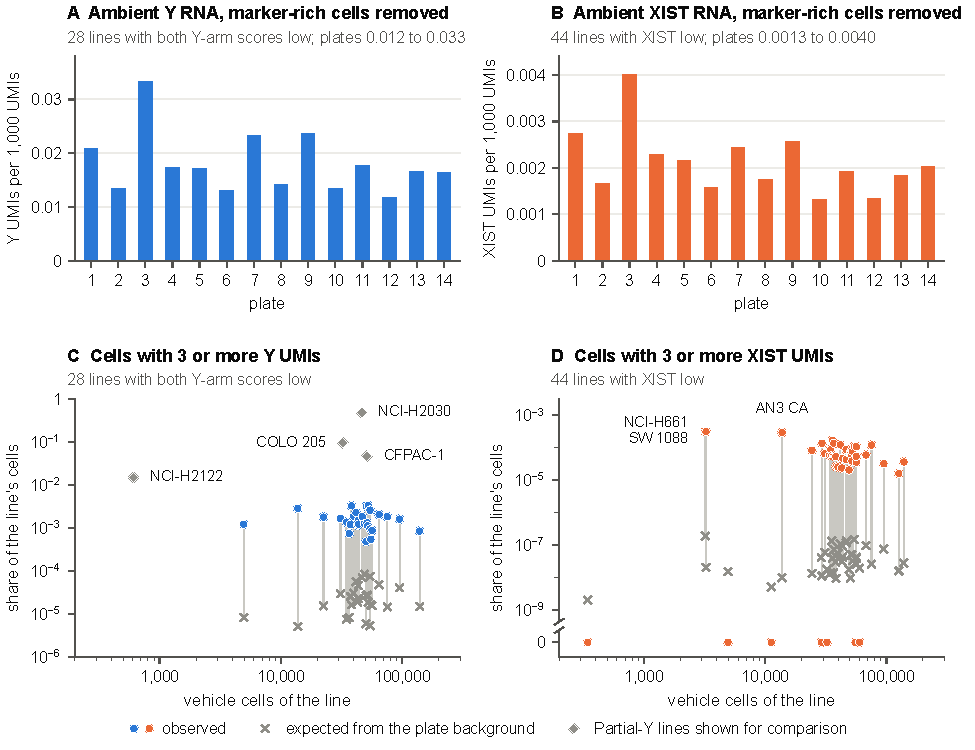
\includegraphics[width=1\linewidth,height=\textheight,keepaspectratio,alt={Figure S1. Ambient RNA and marker-rich cells in Tahoe-100M vehicle cells. One estimate throughout: the first pipeline's, after removing marker-rich cells (3 or more UMIs of the marker). (A) Y UMIs per 1,000 UMIs on each of the 14 plates, pooled over the 28 lines with both Y-arm scores low (0.012 to 0.033). The lines with one Y-arm score high carry their own Y RNA, so they are left out of this background and drawn apart in C. (B) XIST UMIs per 1,000 UMIs over the 44 lines with XIST low (0.0013 to 0.0040). (C, D) Share of a line's vehicle cells with 3 or more Y (C) or XIST (D) UMIs, observed (dots) and expected from the plate background (crosses), against the line's vehicle cells, on logarithmic axes; in D, lines with no such cell sit on a zero row. Marker-rich cells far exceed the ambient expectation (Note S11).}]{figures/figS1_ambient.pdf}
\caption{\textbf{Figure S1. Ambient RNA and marker-rich cells in
Tahoe-100M vehicle cells.} One estimate throughout: the first
pipeline's, after removing marker-rich cells (3 or more UMIs of the
marker). (\textbf{A}) Y UMIs per 1,000 UMIs on each of the 14 plates,
pooled over the 28 lines with both Y-arm scores low (0.012 to 0.033).
The lines with one Y-arm score high carry their own Y RNA, so they are
left out of this background and drawn apart in C. (\textbf{B}) XIST UMIs
per 1,000 UMIs over the 44 lines with XIST low (0.0013 to 0.0040).
(\textbf{C}, \textbf{D}) Share of a line's vehicle cells with 3 or more
Y (C) or XIST (D) UMIs, observed (dots) and expected from the plate
background (crosses), against the line's vehicle cells, on logarithmic
axes; in D, lines with no such cell sit on a zero row. Marker-rich cells
far exceed the ambient expectation (Note S11).}
\end{figure}

\subsection{Note S12. Marker-negative
cells}\label{note-s12.-marker-negative-cells}

The subpopulation analysis covered 22 line to marker pairs. A549 (Y) and
SW48 (XIST) were the only pairs that met the mixture-share criterion in
both implementations. Neither met all criteria in both implementations.

\begin{longtable}[]{@{}
  >{\raggedright\arraybackslash}p{(\linewidth - 8\tabcolsep) * \real{0.3103}}
  >{\raggedright\arraybackslash}p{(\linewidth - 8\tabcolsep) * \real{0.1724}}
  >{\raggedright\arraybackslash}p{(\linewidth - 8\tabcolsep) * \real{0.1724}}
  >{\raggedright\arraybackslash}p{(\linewidth - 8\tabcolsep) * \real{0.1724}}
  >{\raggedright\arraybackslash}p{(\linewidth - 8\tabcolsep) * \real{0.1724}}@{}}
\caption{\textbf{Table S7. Marker-negative shares and mosaic criteria in
Tahoe-100M vehicle cells. Where the pipelines differ, values are local /
the cloud implementation; a single value means they agree at the
precision shown.}}\tabularnewline
\toprule\noalign{}
\begin{minipage}[b]{\linewidth}\raggedright
\end{minipage} & \begin{minipage}[b]{\linewidth}\raggedright
A549, Y
\end{minipage} & \begin{minipage}[b]{\linewidth}\raggedright
SW48, XIST
\end{minipage} & \begin{minipage}[b]{\linewidth}\raggedright
NCI-H460, Y (control)
\end{minipage} & \begin{minipage}[b]{\linewidth}\raggedright
LoVo, Y (control)
\end{minipage} \\
\midrule\noalign{}
\endfirsthead
\toprule\noalign{}
\begin{minipage}[b]{\linewidth}\raggedright
\end{minipage} & \begin{minipage}[b]{\linewidth}\raggedright
A549, Y
\end{minipage} & \begin{minipage}[b]{\linewidth}\raggedright
SW48, XIST
\end{minipage} & \begin{minipage}[b]{\linewidth}\raggedright
NCI-H460, Y (control)
\end{minipage} & \begin{minipage}[b]{\linewidth}\raggedright
LoVo, Y (control)
\end{minipage} \\
\midrule\noalign{}
\endhead
\bottomrule\noalign{}
\endlastfoot
Vehicle cells tested & 60,135 & 22,404 / 22,444 & 126,343 / 126,345 &
67,829 / 67,833 \\
(a) no marker UMI, at least 3,000 UMIs & 0.35 (6,665 cells) & 0.57
(3,924 cells) & 0.04 & 0.15 \\
its bootstrap 95\% interval & 0.34 to 0.36 & 0.55 to 0.58 & 0.03 to 0.04
& 0.14 to 0.15 \\
expected if every cell were positive (Poisson / negative binomial) &
0.02 / 0.06 & 0.10 / 0.40 & 0.01 / 0.03 & 0.06 / 0.14 \\
(a) no marker UMI, at least 8,000 UMIs & 0.19 (145 cells) & 0.33 / 0.31
& 0.00 & 0.02 \\
its bootstrap 95\% interval & 0.13 to 0.26 & 0.24 to 0.43 / 0.22 to 0.41
& 0.00 to 0.00 & 0.02 to 0.03 \\
(b) share at 1,000 UMIs & 0.38 / 0.41 & 0.30 & 0.00 & 0.06 / 0.07 \\
(b) share at 2,000 UMIs & 0.36 / 0.39 & 0.29 / 0.28 & 0.00 & 0.03 \\
(b) share at 4,000 UMIs & 0.33 / 0.36 & 0.28 / 0.27 & 0.00 & 0.01 /
0.02 \\
(b) share at 8,000 UMIs & 0.31 / 0.34 & 0.26 & 0.00 & 0.01 \\
(c) Poisson-mixture share & 0.40 / 0.43 & 0.41 & 0.03 / 0.04 & 0.05 /
0.06 \\
(d) odd against even plates, difference in (b) & 0.03 / 0.02 & 0.05 /
0.06 & 0.00 & 0.00 \\
(e) odds ratio divided by its X-gametolog control & 3.59 / 3.45 & not
applicable & 0.92 / 0.90 & 1.02 / 0.98 \\
(f) margin over the most similar other line & 0.18 / 0.0999 & 0.14 /
0.0766 & 0.20 / 0.1019 & 0.13 / 0.0798 \\
Span of all estimator outputs, both pipelines & 0.19 to 0.43 & 0.26 to
0.57 & 0.00 to 0.04 & 0.01 to 0.15 \\
Verdict, local / the cloud implementation & mosaic / not mosaic & mosaic
/ not mosaic & not mosaic / not mosaic & not mosaic / not mosaic \\
Final verdict & not established & not established & not mosaic & not
mosaic \\
\end{longtable}

Table S7 gives a range across the three estimators and both
implementations. The range summarizes their disagreement and carries no
sampling-interval interpretation. The bootstrap intervals for estimator
(a) resample cells and do not account for the plate structure. Several
markers and controls showed depth-dependent zero counts, so the
estimator outputs do not establish a distinct cell population.

A549's Y-marker zeros exceeded the homogeneous-expression expectation
across all depth bins (Figure S2). The odds ratio for co-occurring zeros
on the two Y arms was 4.06, compared with 1.13 and 1.18 for the
X-gametolog control. A549 was the only Y-tested line to meet the
co-occurrence criterion in either implementation. Of its deep Y-zero
cells, 99.8\% and 99.9\% were nearest A549's own expression centroid.
The atlas had assigned these cells to A549 by genotype. The choice of
background accounted for the two implementations' different A549 mixture
estimates. Including all Y-low lines in the local background reproduced
the cloud estimates, 0.39 for (b) and 0.43 for (c).

For SW48, 0.57 of cells with at least 3,000 UMIs had no observed XIST
UMI, compared with 0.40 expected from the negative-binomial fit to
XIST-positive cells. A post hoc restriction to G1 cells in each depth
quintile altered the observed zero shares by up to 0.02 across A549 and
SW48.

The identity criterion explains the disagreement. The margin over the
closest comparison line was 0.18 versus 0.0999 for A549 and 0.14 versus
0.0766 for SW48, with a requirement of 0.10. The implementations used
different comparison profiles (Note S4). The local implementation also
met the criterion for the two negative controls. The full rule rejected
both controls. With no positive control and disagreement on the identity
check, the data leave both subpopulation claims unresolved.

In ATCC's A549 seed stock, 20 of 50 cells lost one or both Y chromosomes
(95\% CI 0.26 to 0.55). Complete Y loss is a subset of that count, which
gives only an upper bound for that stock. The stock used for Tahoe-100M
may differ.

\begin{figure}
\centering
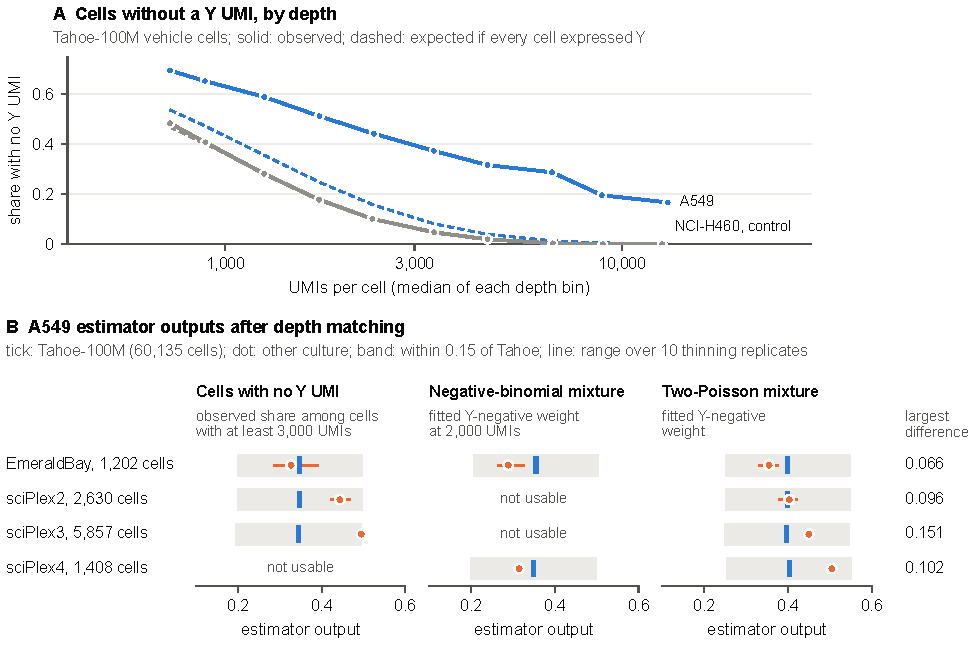
\includegraphics[width=1\linewidth,height=\textheight,keepaspectratio,alt={Figure S2. A549's cells without Y RNA. (A) Share of Tahoe-100M vehicle cells with no Y UMI in each depth bin, against the bin's median UMIs per cell, for A549 (60,135 cells) and the negative-control line NCI-H460 (126,343 cells): observed (solid) and expected if every cell expressed Y at the rate of the line's Y-expressing component (dashed). A549's observed share lies above its expectation at every depth; NCI-H460's follows it. (B) A549's estimator outputs after depth matching, in Tahoe-100M (tick) and in each other culture (dot), one facet per estimator: the share of cells with no Y UMI among cells with at least 3,000 UMIs, or the fitted Y-negative weight of a mixture. The line is the range over 10 thinning replicates, which reflects thinning only; the band spans 0.15 on either side of Tahoe-100M, the comparison tolerance. Only sciPlex3 exceeds it (Note S13).}]{figures/figS2_a549.pdf}
\caption{\textbf{Figure S2. A549's cells without Y RNA.} (\textbf{A})
Share of Tahoe-100M vehicle cells with no Y UMI in each depth bin,
against the bin's median UMIs per cell, for A549 (60,135 cells) and the
negative-control line NCI-H460 (126,343 cells): observed (solid) and
expected if every cell expressed Y at the rate of the line's
Y-expressing component (dashed). A549's observed share lies above its
expectation at every depth; NCI-H460's follows it. (\textbf{B}) A549's
estimator outputs after depth matching, in Tahoe-100M (tick) and in each
other culture (dot), one facet per estimator: the share of cells with no
Y UMI among cells with at least 3,000 UMIs, or the fitted Y-negative
weight of a mixture. The line is the range over 10 thinning replicates,
which reflects thinning only; the band spans 0.15 on either side of
Tahoe-100M, the comparison tolerance. Only sciPlex3 exceeds it (Note
S13).}
\end{figure}

\subsection{Note S13. Depth-matched comparison
results}\label{note-s13.-depth-matched-comparison-results}

Without depth matching, the two-component Poisson estimates for A549
were 0.39 in EmeraldBay and 0.36, 0.45 and 0.50 in sciPlex2, sciPlex3
and sciPlex4. SW48's EmeraldBay estimate was 0.42. The same model
returned an estimate between 0.15 and 0.85 for 18 of 21 Y-low
EmeraldBay lines used as a check, often where the pooled background
exceeded the line's Y rate. A middle-range estimate alone has limited
specificity.

After depth matching, A549's usable estimates were within 0.15 of
Tahoe-100M in EmeraldBay, sciPlex2 and sciPlex4. For sciPlex3, estimator
(a) differed by 0.151, while estimator (c) differed by 0.053. The 95\%
interval for the signed difference under (a), based on deep-cell counts,
spans 0.11 to 0.19 and crosses the tolerance. SW48's two usable
EmeraldBay estimators were within the tolerance. The corresponding
intervals for estimator (a) are −0.10 to 0.06 for A549 and −0.07 to 0.09
for SW48. These post hoc intervals omit variability from thinning. The
LoVo control also crossed the tolerance on estimator (c), with a
difference of 0.154. Sample sizes, estimator availability and the use of
nuclear RNA in sci-Plex limit the comparison. These results give limited
evidence for a stable share across cultures.

\begin{longtable}[]{@{}
  >{\raggedright\arraybackslash}p{(\linewidth - 12\tabcolsep) * \real{0.2500}}
  >{\raggedright\arraybackslash}p{(\linewidth - 12\tabcolsep) * \real{0.1786}}
  >{\raggedright\arraybackslash}p{(\linewidth - 12\tabcolsep) * \real{0.1429}}
  >{\raggedright\arraybackslash}p{(\linewidth - 12\tabcolsep) * \real{0.1071}}
  >{\raggedright\arraybackslash}p{(\linewidth - 12\tabcolsep) * \real{0.1071}}
  >{\raggedright\arraybackslash}p{(\linewidth - 12\tabcolsep) * \real{0.1071}}
  >{\raggedright\arraybackslash}p{(\linewidth - 12\tabcolsep) * \real{0.1071}}@{}}
\caption{\textbf{Table S8. Depth-matched shares, Tahoe against the other
cultures. On the thinned side, the share is the median of 10
replicates.}}\tabularnewline
\toprule\noalign{}
\begin{minipage}[b]{\linewidth}\raggedright
Line, marker, other culture
\end{minipage} & \begin{minipage}[b]{\linewidth}\raggedright
Estimator
\end{minipage} & \begin{minipage}[b]{\linewidth}\raggedright
Thinned side
\end{minipage} & \begin{minipage}[b]{\linewidth}\raggedright
Tahoe
\end{minipage} & \begin{minipage}[b]{\linewidth}\raggedright
Other culture
\end{minipage} & \begin{minipage}[b]{\linewidth}\raggedright
Difference
\end{minipage} & \begin{minipage}[b]{\linewidth}\raggedright
Agrees
\end{minipage} \\
\midrule\noalign{}
\endfirsthead
\toprule\noalign{}
\begin{minipage}[b]{\linewidth}\raggedright
Line, marker, other culture
\end{minipage} & \begin{minipage}[b]{\linewidth}\raggedright
Estimator
\end{minipage} & \begin{minipage}[b]{\linewidth}\raggedright
Thinned side
\end{minipage} & \begin{minipage}[b]{\linewidth}\raggedright
Tahoe
\end{minipage} & \begin{minipage}[b]{\linewidth}\raggedright
Other culture
\end{minipage} & \begin{minipage}[b]{\linewidth}\raggedright
Difference
\end{minipage} & \begin{minipage}[b]{\linewidth}\raggedright
Agrees
\end{minipage} \\
\midrule\noalign{}
\endhead
\bottomrule\noalign{}
\endlastfoot
A549, Y, EmeraldBay & (a) at least 3,000 UMIs & EmeraldBay & 0.348 &
0.327 & 0.021 & yes \\
A549, Y, EmeraldBay & (b) at 2,000 UMIs & EmeraldBay & 0.355 & 0.289 &
0.066 & yes \\
A549, Y, EmeraldBay & (c) & EmeraldBay & 0.400 & 0.355 & 0.045 & yes \\
A549, Y, sciPlex2 & (a) at least 3,000 UMIs & sciPlex2 & 0.348 & 0.443 &
0.096 & yes \\
A549, Y, sciPlex2 & (c) & sciPlex2 & 0.400 & 0.403 & 0.003 & yes \\
A549, Y, sciPlex3 & (a) at least 3,000 UMIs & Tahoe & 0.344 & 0.495 &
0.151 & no \\
A549, Y, sciPlex3 & (c) & Tahoe & 0.397 & 0.450 & 0.053 & yes \\
A549, Y, sciPlex4 & (b) at 2,000 UMIs & Tahoe & 0.349 & 0.315 & 0.034 &
yes \\
A549, Y, sciPlex4 & (c) & Tahoe & 0.403 & 0.505 & 0.102 & yes \\
SW48, XIST, EmeraldBay & (a) at least 3,000 UMIs & EmeraldBay & 0.569 &
0.586 & 0.017 & yes \\
SW48, XIST, EmeraldBay & (c) & EmeraldBay & 0.413 & 0.456 & 0.043 &
yes \\
NCI-H460, Y, EmeraldBay (context) & (a) at least 3,000 UMIs & EmeraldBay
& 0.036 & 0.082 & 0.046 & yes \\
NCI-H460, Y, EmeraldBay (context) & (b) at 2,000 UMIs & EmeraldBay &
0.000 & 0.012 & 0.012 & yes \\
NCI-H460, Y, EmeraldBay (context) & (c) & EmeraldBay & 0.033 & 0.050 &
0.017 & yes \\
LoVo, Y, EmeraldBay (context) & (a) at least 3,000 UMIs & EmeraldBay &
0.146 & 0.239 & 0.093 & yes \\
LoVo, Y, EmeraldBay (context) & (b) at 2,000 UMIs & EmeraldBay & 0.031 &
0.135 & 0.104 & yes \\
LoVo, Y, EmeraldBay (context) & (c) & EmeraldBay & 0.050 & 0.204 & 0.154
& no \\
\end{longtable}

Not used: (a) at 8,000 UMIs in every pair (too few deep cells on one
side after matching); (b) for SW48 and for sciPlex2 (a fit on the
thinned side did not converge or stopped at a bound) and for sciPlex3
(the sciPlex3 fit did not converge or stopped at a bound); and (a) at
3,000 UMIs for sciPlex4 (too few deep cells in sciPlex4).

\subsection{Note S14. STR Amelogenin
comparison}\label{note-s14.-str-amelogenin-comparison}

This descriptive comparison followed the Part B analysis. Note S16
reports the separate cross-stock assessment for lines used in the
response test.

Records. The checked lines are the 50 Tahoe-100M lines and every line of
Table S1 with a Y call from at least one source, 1,102 lines in all; 21
lines of Table S1 have no Y call and were left out. Each record was
fetched by accession from the Cellosaurus API (D11) on 16 November 2026;
the API reported release 57.0 of 22 October 2026, and every request
returned a record. The sex in the fetched record differed from the label
used here for 1 line, LS 174T, which has no label in Part A and is
Female in the record; its EmeraldBay call, ambiguous, would read
XIST-lost under that label.

Amelogenin classes. STR profiles are the reference standard for the
identity of human cell lines (Masters et al.~2001), and Cellosaurus
compiles the published ones (Robin, Capes-Davis and Bairoch 2020).
Amelogenin is the sex marker of STR profiling: it amplifies AMELX on the
X and AMELY on the short arm of the Y (Salido et al.~1992; Sullivan et
al.~1993), so ``X'' means that AMELY was not detected and ``X,Y'' that
it was. Every Amelogenin line of a record was read, and each line was
classed X only if every source reports X, X,Y if every source reports
X,Y, and mixed across sources otherwise. Over all lines checked, 739
were X only, 310 X,Y and 36 mixed; 14 had no Amelogenin result and 3 a
result that could not be classed, and these were not compared. All 50
Tahoe-100M lines were X only (32) or X,Y (18).

Agreement with the Y calls. A Y call agrees with the STR result if X,Y
goes with a Y score above the cut-off, or X only with a score below it.
X,Y with a low Y score (AMELY present, Y not expressed) is called type
A, and X only with a high Y score (AMELY absent, Y expressed) type B.
Agreement was 48 of 50 lines in Tahoe-100M (1 type A, 1 type B), 47 of
52 in EmeraldBay (4 and 1), 3 of 3 for the qualitative sci-Plex calls,
714 of 734 for CCLE (11 and 9) and 1,007 of 1,031 for Cell Model
Passports (17 and 7). The CCLE and Cell Model Passports calls come from
the GDSC2/PRISM external RNA-seq analysis where it has the data and from
the LINCS2020 external RNA-seq analysis otherwise; where both tasks call
the same lines from CCLE, they give the same Y call for 120 of 120.

Tahoe-100M in detail. By state, 13 of the 14 Y-lost lines, all 12
XIST-lost lines, all 5 XX-like lines and A498 were X only, and 17 of the
18 XY lines were X,Y. The type A line is CFPAC-1 (Y-lost; Yp high, Yq
low), which keeps AMELY and expresses its Yp genes. The type B line is
NCI-H596, an XY call with low confidence from 345 cells (Note S9). By
arm pattern, all 12 male-labelled lines with both arm scores low were X
only, and 16 of the 17 with both high were X,Y; of the lines with
exactly one arm score high, COLO 205 and NCI-H2030 were X only and
CFPAC-1 and HCT15 X,Y. NCI-H2030 lacks AMELY although it expresses both
Yp genes strongly, so the Yp score marks which genes are expressed, not
whether the arm is present.

Labels. Over all lines checked, 256 of the 604 male-labelled lines were
X only and 308 X,Y, and 450 of the 458 female-labelled lines were X
only. Of the female-labelled lines, 4 had a Y allele in at least one
source, which conflicts with their label. The comparison flagged 21
lines with a type A discrepancy in at least one source, 13 with a type B
discrepancy and 36 with mixed STR results.

An X-only result means AMELY was not detected in the STR-profiled stock.
Together with a low Y score, this is consistent with loss of the tested
Y region, but single-locus typing does not establish a whole-chromosome
event, copy number or a cell fraction. The STR profiles are from other
stocks and times. Normal Y chromosomes can also lack AMELY (Steinlechner
et al.~2002; Thangaraj, Reddy and Singh 2002). Amelogenin does not
assess XIST expression or X inactivation.

\subsection{Note S15. Data and code
availability}\label{note-s15.-data-and-code-availability}

Table S2 identifies the source datasets and versions. The
\href{https://github.com/MateenahJAHAN/Project-59-CMAP-Sex-Differences\#readme}{public
project repository} contains the paper, figures, earlier CMap and GTEx
notebooks,
\href{https://github.com/MateenahJAHAN/Project-59-CMAP-Sex-Differences/tree/main/verification}{rerun
results}, and
\href{https://github.com/MateenahJAHAN/Project-59-CMAP-Sex-Differences/tree/main/analysis}{analysis
source}. The full Table S1 includes fields derived from provider data.
Input RNA-seq and CMap annotations are available from their providers
under separate terms.

\section{Part B: drug-response
analysis}\label{part-b-drug-response-analysis}

\subsection{Note S16. Part B design}\label{note-s16.-part-b-design}

An AI coding agent helped draft the analysis plan on 15 November 2026.
The plan and code were recorded in private version control before
measured states were joined to drug responses later that day. This
chronology comes from the project's records. The plan was not deposited
in an independent registry. Earlier analyses covered some of the same
data and compounds (Note S19).

The primary and lower-dose panels use the same 41 lines. The Y-only and
XIST-only groups are each compared with lines below both cut-offs. 5
lineages include a direct reference for the Y term and 5 for the XIST
term. Large intestine and soft tissue lack reference lines, so they
inform the coefficients through the additive model. Only skin includes
all three groups. In P2, the Y term used 39 lines (11 vs 28) in 6
lineages, the XIST term 39 lines (12 vs 27) in 6 lineages and annotated
donor sex 31 lines (22 vs 9) in 4 lineages. A direct Y-high versus
XIST-high-only comparison was excluded before the analysis because its
pseudo-label calibration was outside the planned range (0.0180 at p
\textless{} 0.05, compared with 0.03 to 0.07).

\begin{longtable}[]{@{}
  >{\raggedright\arraybackslash}p{(\linewidth - 8\tabcolsep) * \real{0.1728}}
  >{\raggedright\arraybackslash}p{(\linewidth - 8\tabcolsep) * \real{0.0617}}
  >{\raggedright\arraybackslash}p{(\linewidth - 8\tabcolsep) * \real{0.1975}}
  >{\raggedright\arraybackslash}p{(\linewidth - 8\tabcolsep) * \real{0.1975}}
  >{\raggedright\arraybackslash}p{(\linewidth - 8\tabcolsep) * \real{0.3704}}@{}}
\caption{\textbf{Table S9. Primary-panel cell lines by lineage and
expression group.} Y+ denotes Y only and X+ denotes XIST only. The
reference group is below both cut-offs. TP53 status comes from Cell
Model Passports or, for 6 lines, from CCLE. Ploidy comes from Cell Model
Passports.}\tabularnewline
\toprule\noalign{}
\begin{minipage}[b]{\linewidth}\raggedright
Lineage
\end{minipage} & \begin{minipage}[b]{\linewidth}\raggedright
Lines
\end{minipage} & \begin{minipage}[b]{\linewidth}\raggedright
Y+
\end{minipage} & \begin{minipage}[b]{\linewidth}\raggedright
X+
\end{minipage} & \begin{minipage}[b]{\linewidth}\raggedright
Neither (reference)
\end{minipage} \\
\midrule\noalign{}
\endfirsthead
\toprule\noalign{}
\begin{minipage}[b]{\linewidth}\raggedright
Lineage
\end{minipage} & \begin{minipage}[b]{\linewidth}\raggedright
Lines
\end{minipage} & \begin{minipage}[b]{\linewidth}\raggedright
Y+
\end{minipage} & \begin{minipage}[b]{\linewidth}\raggedright
X+
\end{minipage} & \begin{minipage}[b]{\linewidth}\raggedright
Neither (reference)
\end{minipage} \\
\midrule\noalign{}
\endhead
\bottomrule\noalign{}
\endlastfoot
bone & 2 & 1: SKES1 & none & 1: U2OS (XIST-lost) \\
breast & 4 & none & 1: ZR751 & 3: BT474, MDAMB468, T47D (XIST-lost) \\
central nervous system & 3 & 2: GI1, U251MG & none & 1: YH13 (Y-lost) \\
large intestine & 3 & 1: SNU407 & 2: GP2D, HT29 & none \\
lung & 7 & 2: A549, NCIH841 & none & 5: HCC95, NCIH1437, NCIH838
(Y-lost); NCIH1573, NCIH2172 (XIST-lost) \\
ovary & 7 & none & 4: COV434, ES2, OC316, OVK18 & 3: OAW28, OVTOKO,
TOV112D (XIST-lost) \\
prostate & 2 & 1: 22RV1 & none & 1: PC3 (Y-lost) \\
skin & 6 & 2: CJM, IGR37 & 2: A375, MELHO & 2: SH4, SKMEL3
(XIST-lost) \\
soft tissue & 2 & 1: G401 & 1: A204 & none \\
stomach & 3 & none & 2: AGS, MKN45 & 1: IM95 (Y-lost) \\
urinary tract & 2 & none & 1: CAL29 & 1: BC3C (XIST-lost) \\
All 11 lineages & 41 & 10 & 13 & 18 \\
CMap label & & 9 male, 1 with no label & 13 female & 6 male, 12
female \\
TP53 & & 8 mutant, 2 wild type & 6 mutant, 7 wild type & 14 mutant, 4
wild type \\
Ploidy, median (lines with a value) & & 2.28 (9 lines) & 2.87 (10 lines)
& 2.92 (16 lines) \\
\end{longtable}

\textbf{Expression states across stocks.} Part B used calls from CCLE
for 40 lines and from the Broad subset of Cell Model Passports for 1. In
a post hoc comparison, 40 of 40 available Cell Model Passports calls
from the GDSC2/PRISM reference analysis matched the Part B grouping. STR
Amelogenin agreed with the Y grouping for 38 of 38 lines with a clear
X-only or X,Y result (Note S14). Applying the overall CCLE Y cut-off to
each arm separately gave both arms high in all 10 Y+ lines and neither
high in the 18 reference lines and 12 of 13 X+ lines.

The 4 lines shared with Tahoe-100M and EmeraldBay had the same grouping
in those atlases. A549's XIST call varied across sci-Plex experiments
and its Y call remained the same. The sensitivity analysis flagged A549
and the medium-confidence calls for ES2 and GP2D. No source measures
expression states in the LINCS wells, and the small set of shared lines
reflects atlas coverage.

\textbf{Responses and vehicle controls.} The primary LINCS dose label
\texttt{1.11\ uM} includes 8,743 of 9,724 signatures measured at 1.0 µM.
Level-5 signatures are scaled within plates, each of which contains a
single line. This scaling can remove a response shift shared across
compounds. The level-5 DMSO negative control used vehicle signatures
from the same project and time. Level-3 responses subtract the mean of
vehicle wells on each treated plate, with at least two vehicle wells
required.

Permutations. The model without the tested term is fitted, its residuals
are permuted within lineage, and the model is refitted (Freedman-Lane).
Each of the 10,000 permutations gives every line of the panel a random
key, and a compound's available lines are reordered within each lineage
by their keys; this induced permutation means that all compounds and
terms share one set of permutations, so the panel statistic gets its p
value from the same permutations as each compound. A lineage with two
lines can only keep or swap them. In P1 there are 22,680 (Y) and 75,600
(X) distinct relabellings within lineage. The test assumes
exchangeability of the reduced-model residuals within lineage. We used
HC3 studentisation (Winkler et al.~2014). For each compound, lineages
with fewer than two available lines are dropped; the compound is not
tested if fewer than four lines remain, if a group keeps fewer than 3
lines, if there are fewer than 20 relabellings, if the design is
singular or a line has leverage one, or if no residual df is left. With
10,000 permutations, a p value near 0.025 has a Monte Carlo standard
error of about 0.0016.

\textbf{Per-compound covariate check.} The estimate is the 978-gene
coefficient vector of the tested term. The retained fraction is the
inner product of the adjusted vector with the primary vector, divided by
the squared length of the primary vector estimated on all of the
compound's lines; rule 4 holds if it is at least one half both with
ploidy and with the compound's PRISM AUC as a covariate. A separate
ratio on common rows describes how covariate availability affects the
comparison. A compound without a PRISM 19Q4 match, or whose adjusted
model cannot be fitted, does not meet rule 4.

\begin{longtable}[]{@{}
  >{\raggedright\arraybackslash}p{(\linewidth - 6\tabcolsep) * \real{0.2059}}
  >{\raggedright\arraybackslash}p{(\linewidth - 6\tabcolsep) * \real{0.2647}}
  >{\raggedright\arraybackslash}p{(\linewidth - 6\tabcolsep) * \real{0.2647}}
  >{\raggedright\arraybackslash}p{(\linewidth - 6\tabcolsep) * \real{0.2647}}@{}}
\caption{\textbf{Table S10. Part B families of tests and error control.}
Decision rules recorded before measured states were joined to responses.
The plan controls error within the families indicated below. No common
error rate was set across H1 to H3.}\tabularnewline
\toprule\noalign{}
\begin{minipage}[b]{\linewidth}\raggedright
Family
\end{minipage} & \begin{minipage}[b]{\linewidth}\raggedright
Members
\end{minipage} & \begin{minipage}[b]{\linewidth}\raggedright
Procedure and level
\end{minipage} & \begin{minipage}[b]{\linewidth}\raggedright
Outcome
\end{minipage} \\
\midrule\noalign{}
\endfirsthead
\toprule\noalign{}
\begin{minipage}[b]{\linewidth}\raggedright
Family
\end{minipage} & \begin{minipage}[b]{\linewidth}\raggedright
Members
\end{minipage} & \begin{minipage}[b]{\linewidth}\raggedright
Procedure and level
\end{minipage} & \begin{minipage}[b]{\linewidth}\raggedright
Outcome
\end{minipage} \\
\midrule\noalign{}
\endhead
\bottomrule\noalign{}
\endlastfoot
H1, panel level & Y and X terms in P1 & Bonferroni over the two terms:
each rejected at p \textless{} 0.025 & neither rejected \\
H2, per compound & 114 testable compounds per term in P1. Of these, 48
met the eligibility criteria. The exclusions included 44 previously
studied compounds and 28 without a PRISM 19Q4 match (overlapping
exclusions) & Benjamini-Hochberg within P1 and term, q \textless{} 0.1,
and rules 2 to 4 & no finding \\
H3, pooled magnitude & Y and X terms in P1, level 3 & estimation; a
difference only if the 95\% CI excludes zero, per term and without
adjustment; an equivalence claim requires a label-free chance of at
least 0.8 & no difference declared; no equivalence claim \\
H4, annotated sex & annotated term in P1 & the tests of H1 to H3,
without claims of their own & p = 0.5544; no finding \\
Vehicle control & DMSO under each term & a reading rule if the DMSO p is
below 0.05 & applies to X; no H1 result for it to qualify \\
Secondary readouts & CollecTRI TF layer, focused Lopes-Ramos TFs,
X-linked landmark score, in P1, P1b and P2 & Benjamini-Hochberg across
compounds within the TF layer; single tests otherwise; labelled
secondary & no P1 readout below 0.05 \\
P1b and P2 & H1 to H3 for each term & as in P1, reported without claims
& no panel p below 0.025 \\
Leads L1 to L4 & four P1 tests; L3 also in P2, outside the Holm family &
0.05 each, with and without Holm over the four P1 tests & L4 below 0.05
with Holm (0.0160; 0.0200 if the P2 test were a fifth member); L3 below
0.05 without Holm only \\
Sensitivity analyses S1 to S12 & one change each & reported against
0.025, without claims & none below \\
Checks before joining states & AMG-232 positive control, calibration and
E3 precision & Stop rules for the primary analysis & The compound-level
AMG-232 control passed in P1. The panel-wide TP53 benchmark on the
analysis-specific line set did not reach the panel threshold (Note
S17). \\
\end{longtable}

\begin{longtable}[]{@{}
  >{\raggedright\arraybackslash}p{(\linewidth - 2\tabcolsep) * \real{0.5882}}
  >{\raggedright\arraybackslash}p{(\linewidth - 2\tabcolsep) * \real{0.4118}}@{}}
\caption{\textbf{Table S11. Part B analyses added after the main
result.}}\tabularnewline
\toprule\noalign{}
\begin{minipage}[b]{\linewidth}\raggedright
Analysis
\end{minipage} & \begin{minipage}[b]{\linewidth}\raggedright
Scope
\end{minipage} \\
\midrule\noalign{}
\endfirsthead
\toprule\noalign{}
\begin{minipage}[b]{\linewidth}\raggedright
Analysis
\end{minipage} & \begin{minipage}[b]{\linewidth}\raggedright
Scope
\end{minipage} \\
\midrule\noalign{}
\endhead
\bottomrule\noalign{}
\endlastfoot
Vehicle-referenced responses & P1 follow-up extended to P1b and P2 after
the first follow-up results. A separate diagnostic assessed shared
structure in the level-5 response after vehicle subtraction (Note
S18). \\
Idarubicin & An analysis of the selected dose and time was extended to
all available conditions (Note S18). \\
Design diagnostics & Panel calibration, planted-effect simulations,
interval coverage, TP53 benchmark, weak templates and expression-state
sensitivity (Note S17, Figure S3). \\
Cross-stock expression states & Comparison of states used in Part B with
other RNA-seq datasets, vehicle-cell atlases and STR Amelogenin records
(Note S16). \\
\end{longtable}

\subsection{Note S17. Part B results, sensitivity and
power}\label{note-s17.-part-b-results-sensitivity-and-power}

\textbf{Primary results.} Of the 115 compounds in P1, 114 could be
tested. AZD-8055 lacked enough eligible lines. The earlier list included
45 of the 115 compounds and 44 of the tested compounds (Note S19). The
panel statistics were 0.663 for Y (p = 0.7231) and 0.747 for XIST (p =
0.1127). Neither met the threshold of 0.025. The XIST term had 11
compounds with p \textless{} 0.05, above the discovery-count threshold
of 10. The XIST DMSO control gave p = 0.0323. The design chance of an
interval wholly inside the prespecified margin was 0.090 for Y and 0.255
for XIST, below the planned minimum of 0.8 for each term (Table S12).

\textbf{Controls.} On the positive-control line set, AMG-232 ranked 1 of
114 by the TP53 contrast (p = 0.0008). Its CDKN1A coefficient for mutant
minus wild-type TP53 was −3.99 on level 5 and retained its direction on
level 3 (−1.965). The mean share of compounds at p \textless{} 0.05 in
the calibration draws ranged from 0.0396 to 0.0446. The median 90\% E3
interval half-width in precision simulations was 18.5\% for Y and 17.0\%
for XIST, relative to mean response size.

\textbf{Design diagnostics.} These analyses followed the primary results
(Table S11).

\begin{itemize}
\tightlist
\item
  Size of the panel-level test. The calibration check concerns
  per-compound p values. In the same pseudo-label draws (2,000
  permutations each), we counted the number of pseudo-labellings with a
  panel p below 0.05 and below 0.025: in P1, of 200, 0 and 0 (Y), 2 and
  1 (X), 1 and 1 (annotated); in the same order, in P1b, of 100, 2 and
  1, 3 and 1, 2 and 1; in P2, of 100, 5 and 3, 3 and 1, 4 and 3. Over
  1,000 fresh pseudo-labellings in P1 (2,000 permutations each), the
  panel p fell below 0.05 in 13 of 1,000 (Y) and 6 of 1,000 (X), and
  below 0.025 in 3 of 1,000 and 5 of 1,000; the exact upper 95\% bounds
  of the shares at 0.025 are 0.009 and 0.012, so the test is
  conservative at its decision level. The per-compound shares at p
  \textless{} 0.05 were 0.0440 and 0.0417.
\item
  Why the panel-level test is conservative. On the first 200 of those
  pseudo-labellings the test was rerun with fewer terms. With lineage
  and the tested term alone, permuting residuals within lineage is the
  same as relabelling the lines, so that test is exact: its mean panel p
  was 0.507 (Y) and 0.495 (X), consistent with the one half of a uniform
  p.~Without TP53 it was 0.539 and 0.549, and in the primary model 0.561
  and 0.577. Paired on these pseudo-labellings, the frozen model's panel
  p exceeds that with the tested term alone by 0.054 (SE 0.012) for Y
  and 0.082 (SE 0.011) for X. The covariates of the Freedman-Lane
  reduced model, TP53 and the other state term, therefore place the
  permutation null of the panel statistic above the statistic's
  distribution under labels that carry no information.
\item
  TP53 status as a benchmark. On the factorial line set and under the
  primary testability rules, TP53 status gives a panel statistic of
  0.811 (p = 0.1424), with 11 compounds at p \textless{} 0.05 and 6 at q
  \textless{} 0.1 (AMG-232, daunorubicin, camptothecin, mitoxantrone,
  ceritinib and mitomycin-c), over 32 lines (21 mutant, 11 wild type) in
  7 lineages. The initial control panel gave p = 0.0039. Only 25 lines
  were shared, with consistent TP53 annotations across both sets.
  AMG-232 ranks 1 of 114 (p = 0.0004, q = 0.0228), with E2 −162.2\%
  (95\% CI −249.6 to −74.8), an on/off pharmacological effect. The
  pooled response-size difference for TP53 status, mutant minus wild
  type, is −4.5\% on level 3 (95\% CI −18.0 to 9.1) and −3.6\% on level
  5 (95\% CI −16.8 to 9.7), and −4.1\% on level 3 in the PC1 gate's line
  set (95\% CI −18.9 to 10.7). A known modifier of a handful of
  compounds thus moves the pooled response size by a few percent, far
  from the ±20\% margin; the panel-level test misses it on this line
  set, while the per-compound tests find it. In P1b and P2 the TP53
  panel p is 0.3490 and 0.1350.
\item
  Detectable effects from model-based intervals. For an interval with
  half-width h on d residual df, the implied standard error is h divided
  by the t quantile at 95\% on d df, and the effect that a two-sided
  test at 0.05 detects with 80\% power is about that standard error
  times the sum of the t quantiles for the test and for the power. For
  E3 on level 3 the standard errors are 10.6 (Y) and 10.4 (X) percentage
  points, so the detectable effects are about 30.9\% and 30.2\%, with
  approximate power 0.44 and 0.46 at the ±20\% margin; on level 5 they
  are 18.8\% and 23.8\%. The median detectable E2 is 96.3\% (Y) and
  92.6\% (X), with power 0.31 and 0.33 at 50\%, and the median
  detectable E1 1.62 and 1.59 SD per gene, with power 0.41 and 0.42 at 1
  SD. These approximations ignore multiplicity and take the HC3 standard
  errors at face value; the simulation below is the direct estimate.
\item
  E1 and E2 are marginal intervals, one per gene or compound, not joint
  bounds. The quartiles of the per-compound E2 90\% half-width are 41.3,
  56.4 and 76.2\% (Y) and 40.1, 54.3 and 77.1\% (X); 64 of 114 compounds
  (Y) and 69 of 114 (X) have a half-width above the 50\% of interest.
  The median E1 half-width exceeds 1 SD in 30 of 114 compounds (Y) and
  19 of 114 (X).
\item
  Initial spike-in analysis (P1, 44 lines, level 5, one compound). For a
  shape effect of 1.5 SD in 5\% of the landmarks, the share of spike-ins
  at p \textless{} 0.05 was 0.875 for Y, but at q \textless{} 0.1 it was
  0.11 (Y) and 0.11 (X). Doubling one compound's response size gave 0.41
  (Y) and 0.42 (X).
\item
  Planted-effect power on the final design (Figure S3). Lines of the
  41-line set were given random labels with the real group sizes in each
  lineage, an effect was planted in the real responses of the labelled
  group, which keeps the missing values and the dependence among genes,
  compounds and lines, and the primary tests were run 1,000 times per
  scenario with 2,000 permutations. A pooled difference planted at 10\%,
  20\%, 30\% and 50\% was declared on level 3 in 0.075, 0.301, 0.628 and
  0.992 of runs for Y and 0.106, 0.396, 0.766 and 0.995 for X; at a
  planted E3 of exactly 20\%, interpolated, the level-3 rate is 0.340
  (Y) and 0.409 (X). At 20\% the panel-level test rejected in 0.059 (Y)
  and 0.028 (X) of runs, and at 50\% in 0.751 and 0.632. With no planted
  effect, a level-3 difference was declared in 0.023 (Y) and 0.026 (X)
  of runs. A response larger by 50\% in 1, 6 or 23 compounds put at
  least one planted compound at q \textless{} 0.1 in 0.016, 0.118 and
  0.357 of runs for Y and 0.014, 0.112 and 0.352 for X; one residual SD
  added to 49 landmark genes in 23 compounds did so in 0.091 (Y) and
  0.082 (X). H2 rule 4 was not applied, so the per-compound rates are
  upper bounds on finding rates; with 2,000 permutations a single
  compound reaches q \textless{} 0.1 only if no permutation statistic
  reaches it, so the single-compound rates are lower bounds for the
  run's 10,000 permutations.
\item
  Coverage of the intervals. With random labels and no planted effect,
  the level-3 E3 intervals contained the true value in 0.958 (Y) and
  0.944 (X) of runs at 90\%, and in 0.977 and 0.974 at 95\%; with a
  planted 20\% effect, in 0.960 and 0.940 at 90\%. The per-compound E2
  90\% intervals contained it in 0.956 (Y) and 0.953 (X), and those of
  weak-template compounds in 0.960 and 0.955. The reason is that the HC3
  standard error of E3 was 1.32 (Y) and 1.20 (X) times the actual spread
  of the estimate on level 3, and 1.35 and 1.18 on level 5. The
  intervals hold their level, also with weak templates, but are wider
  than they need be, so they declare a difference less often than
  nominal; this is also why the simulated power at 20\% is below the
  approximation above. In the initial pseudo-label draws, the level-3
  HC3 90\% intervals covered zero in 0.955 (Y) and 0.955 (X) of 200
  pseudo-labellings, and on level 5 they excluded zero in 2.5\% to 4.5\%
  of draws, against a nominal 10\%.
\item
  Weak templates. Response size divides by the squared length of the
  compound's mean response, which is small for weakly active compounds.
  With the weak-template quarter left out (86 of 115 compounds kept), E3
  on level 3 is −7.7\% for Y (95\% CI −28.1 to 12.8) and 2.7\% for X
  (95\% CI −17.9 to 23.3); with only the compounds above the median
  activity (57 of 115), 2.3\% and 11.3\%. On level 5 the same variants
  give 6.2\% and 9.4\% for Y. The Y-term estimate on level 3 moves
  toward zero, and changes sign, as weakly active compounds are left
  out, and 0 of 12 variants declare a difference.
\item
  Misclassification. With the 3 flagged lines (GP2D, A549 and ES2; Note
  S16) excluded, E3 on level 3 is −11.2\% for Y (95\% CI −38.1 to 15.7;
  38 lines (9 vs 29)) and 3.1\% for X (95\% CI −20.1 to 26.4). Over
  every exclusion and reassignment variant, E3 ranges over −11.3 to
  −10.4\% (Y) and 1.5 to 3.9\% (X) on level 3, and 6.7 to 10.4\% and 4.2
  to 6.5\% on level 5; 0 of 32 variants declare a difference, and the
  panel-level test without the flagged lines gives p = 0.6364 (Y) and
  0.3549 (X). Misclassification of the other kind, a labelled line that
  does not carry the effect, biases the estimate toward zero: with a
  20\% effect planted in all but one labelled line, E3 on level 3 keeps
  0.91 (Y) and 0.93 (X) of the planted value, and with two such lines
  0.81 and 0.86.
\item
  Replicate structure. Of the 9,724 P1 signatures at the
  \texttt{1.11\ uM} label, over all lines, 3,739 were built from two or
  more replicate wells. In the line set, 344 of the 4,519
  line-by-compound responses (7.6\%) include such a signature, and no
  compound has more than 3 such lines, which is why S11 tested no
  compound. The residual SD of E1 therefore includes the technical noise
  of single wells.
\end{itemize}

\begin{figure}
\centering
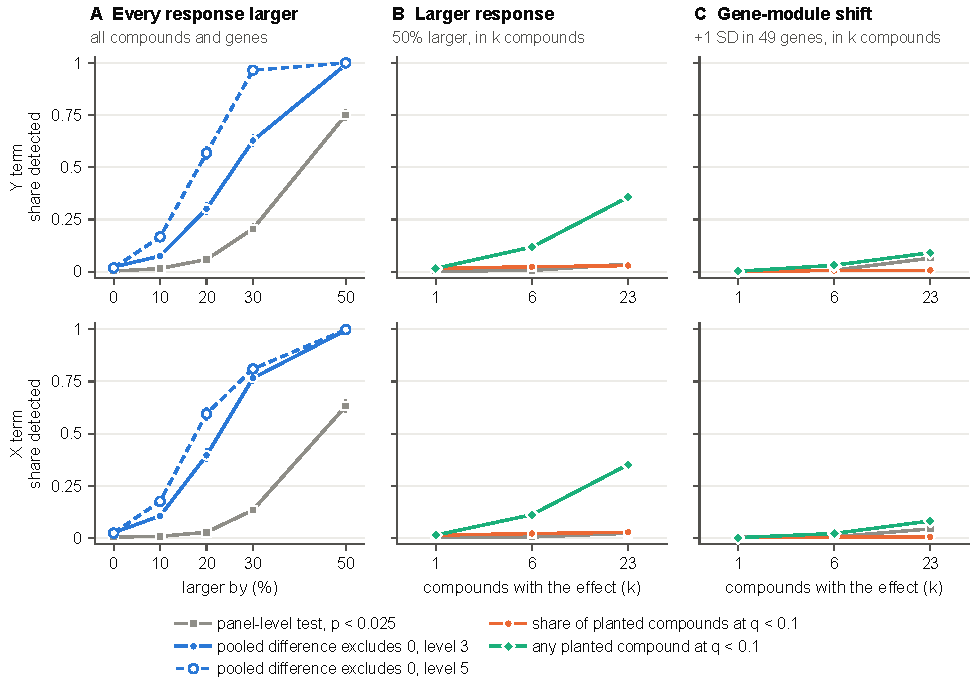
\includegraphics[width=1\linewidth,height=\textheight,keepaspectratio,alt={Figure S3. Power of the Part B tests for effects planted in real responses. Lines of the primary panel were given random labels with the real group sizes in each lineage, an effect was planted in the responses of the labelled group, and the tests were run with the same analysis code, 1,000 times per point with 2,000 permutations. Rows: the Y and X terms. (A) Every response of the group larger by the percentage shown. (B) A response larger by 50\% to k compounds. (C) One residual standard deviation added to 49 landmark genes in k compounds. Each point is the share of runs that detected the effect, with its 95\% interval: grey, the panel-level test at p \textless{} 0.025; blue, the pooled response-size difference with a 95\% interval that excludes zero (filled, level 3; open, level 5); orange, the share of planted compounds at q \textless{} 0.1, where q is the p value adjusted for the false-discovery rate; green, at least one planted compound at q \textless{} 0.1. With no planted effect, the points show how often each test fires by chance. Effects of other shapes could be easier or harder to detect.}]{figures/figS3_power.pdf}
\caption{\textbf{Figure S3. Power of the Part B tests for effects
planted in real responses.} Lines of the primary panel were given random
labels with the real group sizes in each lineage, an effect was planted
in the responses of the labelled group, and the tests were run with the
same analysis code, 1,000 times per point with 2,000 permutations. Rows:
the Y and X terms. (\textbf{A}) Every response of the group larger by
the percentage shown. (\textbf{B}) A response larger by 50\% to k
compounds. (\textbf{C}) One residual standard deviation added to 49
landmark genes in k compounds. Each point is the share of runs that
detected the effect, with its 95\% interval: grey, the panel-level test
at p \textless{} 0.025; blue, the pooled response-size difference with a
95\% interval that excludes zero (filled, level 3; open, level 5);
orange, the share of planted compounds at q \textless{} 0.1, where q is
the p value adjusted for the false-discovery rate; green, at least one
planted compound at q \textless{} 0.1. With no planted effect, the
points show how often each test fires by chance. Effects of other shapes
could be easier or harder to detect.}
\end{figure}

H1 beside other exposures (E5, the excess panel statistic). The excess
of the panel statistic over its null median is −0.022 (Y), 0.040 (X) and
−0.006 (annotated), against 0.032 for TP53 status and −0.0004 for the
within-lineage ploidy split (p = 0.5044). The Y statistic lies inside
the 5th to 95th percentiles of random partitions with the same
per-lineage sizes (0.632 to 0.724), and the X statistic, 0.747, sits at
the 95th percentile of its random partitions (0.667 to 0.748). The DMSO
p value in the separate TP53 control model was 0.0439. Over the 66
compounds complete over the line set, p is 0.9015 (Y) and 0.1841 (X);
over the 56 compounds above the median activity, 0.5205 (Y) and 0.1286
(X).

H2. The compounds at p \textless{} 0.05, with p in brackets and none at
q \textless{} 0.1, are, for Y, cabozantinib (0.016), epirubicin (0.025),
YM-155 (0.025), camptothecin (0.028), lomerizine (0.030), idarubicin
(0.045); for X, axitinib (0.006), idarubicin (0.007), marbofloxacin
(0.015), lapatinib (0.019), CV-1808 (0.023), CGS-15943 (0.027), AZ-628
(0.029), barasertib-HQPA (0.029), raloxifene (0.034), daunorubicin
(0.037), epirubicin (0.048). Rule 2 holds for 5 compounds for each term.
Gene-level tests for the top-ranked compound of each term, YM-155, found
0 genes at q \textless{} 0.1 for Y and 0 for X. The BH family holds all
114 tested compounds, but only 48 could become findings (Table S10).
Among the compounds above the median activity, the smallest q is 0.515
(Y) and 0.370 (X). Rule 2 ranks raw T\textsubscript{c}, whose null mean
grows as a compound's residual df falls, so it favours compounds tested
in fewer lines (for example YM-155, ranked first for both terms over 22
lines, 4 of which express Y genes, with 11 residual df); a rank by p, or
by T\textsubscript{c} standardised to its own null, would avoid this in
a future design.

H3. Table S12 gives E3 for every panel, term and scale. The estimates
depend on the scale: for Y, they are negative on level 3 in all three
panels but positive on level 5 in P1 and P1b, and for X the sign differs
between scales in P2. Response size S correlates at r 0.231 between the
two scales across P1 lines, and on level 3 the median P1 line sits on 1
plate, with a plate-to-plate intraclass correlation of 0.389 for
response size, so level-3 response size is partly a property of the
plate. The primary X interval (90\% CI −16.1 to 19.3) lies inside ±20\%,
so a two one-sided test at the 0.05 level would place the X-term
difference within the margin on this scale; the plan's rule for an
equivalence claim also needs a design chance of at least 0.8, which is
0.255, so no equivalence claim is made. With each line's PRISM viability
score as a covariate (the line's mean over the P1 compounds of the
z-scored PRISM AUC), over the 40 lines that have one, E3 is −11.5\% for
Y (90\% CI −31.3 to 8.3) and 2.2\% for X (90\% CI −19.0 to 23.4).

\begin{longtable}[]{@{}
  >{\raggedright\arraybackslash}p{(\linewidth - 10\tabcolsep) * \real{0.1034}}
  >{\raggedright\arraybackslash}p{(\linewidth - 10\tabcolsep) * \real{0.1034}}
  >{\raggedright\arraybackslash}p{(\linewidth - 10\tabcolsep) * \real{0.0862}}
  >{\raggedright\arraybackslash}p{(\linewidth - 10\tabcolsep) * \real{0.0862}}
  >{\raggedright\arraybackslash}p{(\linewidth - 10\tabcolsep) * \real{0.3103}}
  >{\raggedright\arraybackslash}p{(\linewidth - 10\tabcolsep) * \real{0.3103}}@{}}
\caption{\textbf{Table S12. Part B: E3, the pooled response-size
difference, for every panel, term and scale.} Each cell gives E3 in
percent of the mean S of the lines in the model, with its 90\% CI and
then its 95\% CI (model-based: HC3, t on the residual df, mean S treated
as fixed). Level 3 is each treated well minus the mean of its plate's
DMSO wells; level 5 is CMap's consensus z-scores. Only P1 on level 3
carries decision rules (H3); level 5 is S12; annotated sex (H4), P1b and
P2 make no claims, and P1b and P2 have no positive control that passed
before the freeze. One interval excludes zero at 90\% but not at 95\%:
annotated sex on level 5 in P1.}\tabularnewline
\toprule\noalign{}
\begin{minipage}[b]{\linewidth}\raggedright
Panel
\end{minipage} & \begin{minipage}[b]{\linewidth}\raggedright
Term
\end{minipage} & \begin{minipage}[b]{\linewidth}\raggedright
Lines (df)
\end{minipage} & \begin{minipage}[b]{\linewidth}\raggedright
Mean S, level 3; level 5
\end{minipage} & \begin{minipage}[b]{\linewidth}\raggedright
Level 3
\end{minipage} & \begin{minipage}[b]{\linewidth}\raggedright
Level 5
\end{minipage} \\
\midrule\noalign{}
\endfirsthead
\toprule\noalign{}
\begin{minipage}[b]{\linewidth}\raggedright
Panel
\end{minipage} & \begin{minipage}[b]{\linewidth}\raggedright
Term
\end{minipage} & \begin{minipage}[b]{\linewidth}\raggedright
Lines (df)
\end{minipage} & \begin{minipage}[b]{\linewidth}\raggedright
Mean S, level 3; level 5
\end{minipage} & \begin{minipage}[b]{\linewidth}\raggedright
Level 3
\end{minipage} & \begin{minipage}[b]{\linewidth}\raggedright
Level 5
\end{minipage} \\
\midrule\noalign{}
\endhead
\bottomrule\noalign{}
\endlastfoot
P1 & Y & 41 (27) & 0.764; 0.788 & −11.0 (−29.1 to 7.1; −32.8 to 10.8) &
8.0 (−3.0 to 18.9; −5.3 to 21.2) \\
P1 & X & 41 (27) & 0.764; 0.788 & 1.6 (−16.1 to 19.3; −19.7 to 22.9) &
6.3 (−7.7 to 20.2; −10.5 to 23.1) \\
P1 & annotated & 25 (17) & 0.772; 0.805 & −6.0 (−27.3 to 15.3; −31.9 to
19.8) & 11.6 (0.6 to 22.6; −1.8 to 25.0) \\
P1b & Y & 41 (27) & 0.697; 0.768 & −22.4 (−47.8 to 3.0; −53.0 to 8.2) &
5.2 (−5.8 to 16.1; −8.1 to 18.4) \\
P1b & X & 41 (27) & 0.697; 0.768 & 1.3 (−21.4 to 23.9; −26.0 to 28.5) &
0.4 (−14.0 to 14.9; −17.0 to 17.9) \\
P1b & annotated & 25 (17) & 0.754; 0.804 & −16.4 (−43.9 to 11.2; −49.8
to 17.1) & 7.7 (−3.0 to 18.4; −5.3 to 20.6) \\
P2 & Y & 39 (30) & 0.725; 0.838 & −23.2 (−50.5 to 4.1; −56.1 to 9.7) &
−1.4 (−13.9 to 11.1; −16.5 to 13.6) \\
P2 & X & 39 (30) & 0.725; 0.838 & −9.8 (−38.5 to 19.0; −44.4 to 24.8) &
4.1 (−7.2 to 15.5; −9.5 to 17.8) \\
P2 & annotated & 31 (25) & 0.724; 0.848 & 0.9 (−33.1 to 34.9; −40.0 to
41.9) & −11.1 (−23.0 to 0.8; −25.5 to 3.2) \\
P1, PRISM AUC as a covariate & Y & 40 (25) & & −11.5 (−31.3 to 8.3;
−35.3 to 12.4) & \\
P1, PRISM AUC as a covariate & X & 40 (25) & & 2.2 (−19.0 to 23.4; −23.3
to 27.8) & \\
P1, PRISM AUC as a covariate & annotated & 23 (14) & & −4.8 (−30.4 to
20.8; −35.9 to 26.3) & \\
\end{longtable}

H4. In the annotated set, 24 of 25 lines have a state call. Among lines
annotated male, the share that expresses Y genes is 0.545 and the share
that expresses XIST is 0.091; among lines annotated female, the shares
are 0.077 and 0.538. Of the lines annotated male, 5 of 11 have a Y score
below the cut-off, so the annotated contrast is a diluted version of the
state contrast, over fewer lines.

Secondary family. No secondary readout in P1 has p below 0.05. - The
CollecTRI TF layer uses the 194 single TFs with at least 10 landmark
targets (Müller-Dott et al.~2023); it runs the per-compound test on TF
activities and applies Benjamini-Hochberg across compounds. For Y it
gives p = 0.7046, with 0 compounds at q \textless{} 0.1; for X, p =
0.2419, with 0 compounds at q \textless{} 0.1. The 25 CollecTRI
complexes are reported descriptively, with panel statistics of 0.546 (Y)
and 0.653 (X) and no p value. - The focused one-sided test of TFs with
sex-biased targeting (Lopes-Ramos et al.~2020) uses the 42 of the 43
Lopes-Ramos TFs that have a PANDA-LCL regulon (Glass et al.~2013;
Sonawane et al.~2017; data set: Sonawane 2017). MYBL1 is not testable.
For Y the test gives p = 0.3079 (competitive p = 0.3234); for X, p =
0.3269 (competitive p = 0.7091). These regulons come from lymphoblastoid
cells, and the sex-biased targeting from tissues in vivo, so the test's
rationale for carcinoma lines in culture is weak. Earlier tests on the
old panel are listed in Note S19. - For the X term, the centred X-linked
landmark score over 30 X-linked landmark genes is −0.018 in P1
(two-sided p = 0.3603). In P2 it is 0.084 (two-sided p = 0.0072;
competitive p = 0.0071), one of the 26 secondary tests (Table S10). P2
makes no claims of its own, and this readout is secondary.

Leads. The leads use E2 on level 5, with the Freedman-Lane p, one-sided
where the plan gives a direction. Saha et al.~2024 derived L1 to L3 from
lung adenocarcinoma networks checked against drug sensitivity, so these
tests, of L1000 response size across lineages by measured state, are not
repeats of that work. - L4, idarubicin, Y term, two-sided: p = 0.0040
over 33 lines (8 that express Y genes, 11 that express XIST and 14 that
express neither, in 10 lineages, with 20 residual df), and Holm-adjusted
p = 0.0160. E2 is 34.9\% (90\% CI 14.9 to 55.0) of the mean S. The
X-term E2 for idarubicin is 28.1\% (90\% CI 10.4 to 45.8), with shape p
= 0.0066, the second-smallest X p.~Epirubicin has E2 37.5\% (Y; 90\% CI
−3.9 to 78.8) and 50.8\% (X; 3.3 to 98.2), and daunorubicin 86.1\% (Y;
−2.2 to 174.5) and 96.1\% (X; 28.4 to 163.7). The same sign under both
terms points to the shared reference group as much as to either marker;
correlates of marker loss that are not in the model, such as aneuploidy
or proliferation, could produce it. Earlier analyses of idarubicin are
listed in Note S19. In H2, its Y-term shape test has p = 0.0446, q =
0.847 and rank 3, so it is not a finding. - L3, vorinostat, X term,
one-sided (larger in lines that express XIST): p = 0.0465 in P1, with E2
17.7\% (90\% CI −3.8 to 39.2), and p = 0.0404 in P2, with E2 19.4\%
(90\% CI −1.1 to 39.8). Its Holm-adjusted p in P1 is 0.1395, so it is
below 0.05 without Holm and not with it. The P2 test is outside the Holm
family of four. - L1, trametinib, X term, one-sided (larger in lines
that express XIST): p = 0.1503. L2, panobinostat, Y term, one-sided
(larger in lines that express Y genes): p = 0.0883.

P1b and P2. These panels make no claims of their own, and neither has a
positive control that passed before the freeze: PC1 fails at 0.1 µM, and
no P2 control passed. No panel p is below 0.025: in P1b, p is 0.7659
(Y), 0.1311 (X) and 0.7251 (annotated sex); in P2, it is 0.4266, 0.3290
and 0.4892. In each panel and term, the count of compounds at p
\textless{} 0.05 is at or below the panel's own pseudo-label 95th
percentile. In P1b, the counts are 7, 8 and 2, against 11, 11 and 10; in
P2, they are 12, 11 and 8, against 20.1, 18.05 and 19.05. No E3
difference is declared in either panel (Table S12).

Positive shape correlation and the same E2 direction across P1 and P2
were observed for 2 of 20 shared compounds for Y and 0 of 20 for XIST.
AZD-8055 had 31 P1 lines at the \texttt{1.11\ uM} label. Of these, 2
were in the primary line set and 0 remained after the lineage
restriction.

Sensitivity analyses. No sensitivity analysis that could be run rejects
either term at p \textless{} 0.025 (Table S13). The smallest panel p is
0.0929, for the X term under S10. S4 is P1b, which lacks a passing
positive control, so its null adds little. S2 dropped no P1 line, so in
P1 it equals the primary analysis; in P2 it gives p = 0.4324 (Y) and
0.4046 (X). S12 is in Table S12.

S11 could not be analysed. No compound had enough lines for the model
when each signature was required to have two or more replicates. A
diagnostic after the run applied the same testability rule to line
membership and group codes, and computed no test statistic. It
reproduced the primary analysis, with 114 compounds testable, and found
all 115 compounds untestable under S11, with too few lines. The median
number of analysis-set lines per compound with such a signature is 3.

Across compounds, E2 compared with the compounds' PRISM viability effect
gives, for Y, Spearman −0.050 over 86 compounds (relabelling 95\% range
−0.306 to 0.092; p = 0.831); for X, Spearman −0.291 over 86 compounds
(relabelling 95\% range −0.409 to 0.042; p = 0.191). The relabelling
nulls of these correlations are not centred at zero (means −0.13 and
−0.19), so each is read against its own range.

\begin{longtable}[]{@{}
  >{\raggedright\arraybackslash}p{(\linewidth - 6\tabcolsep) * \real{0.1250}}
  >{\raggedright\arraybackslash}p{(\linewidth - 6\tabcolsep) * \real{0.3750}}
  >{\raggedright\arraybackslash}p{(\linewidth - 6\tabcolsep) * \real{0.2500}}
  >{\raggedright\arraybackslash}p{(\linewidth - 6\tabcolsep) * \real{0.2500}}@{}}
\caption{\textbf{Table S13. Part B sensitivity analyses: the H1 panel p
in P1 under each change.} Each cell gives the lines (group 1 vs the rest
of the model) and the panel p; group 1 is the lines that express Y
genes, or XIST, and the rest include the other term's group, as in the
main model. 114 compounds were tested unless the cell says otherwise.
S12 is in Table S12.}\tabularnewline
\toprule\noalign{}
\begin{minipage}[b]{\linewidth}\raggedright
Analysis
\end{minipage} & \begin{minipage}[b]{\linewidth}\raggedright
Change from the primary analysis
\end{minipage} & \begin{minipage}[b]{\linewidth}\raggedright
Y term
\end{minipage} & \begin{minipage}[b]{\linewidth}\raggedright
X term
\end{minipage} \\
\midrule\noalign{}
\endfirsthead
\toprule\noalign{}
\begin{minipage}[b]{\linewidth}\raggedright
Analysis
\end{minipage} & \begin{minipage}[b]{\linewidth}\raggedright
Change from the primary analysis
\end{minipage} & \begin{minipage}[b]{\linewidth}\raggedright
Y term
\end{minipage} & \begin{minipage}[b]{\linewidth}\raggedright
X term
\end{minipage} \\
\midrule\noalign{}
\endhead
\bottomrule\noalign{}
\endlastfoot
S1 & earlier 44-line set & 44 (11 vs 33); p = 0.6481 & 44 (14 vs 30); p
= 0.1903 \\
S1 & GDSC2/PRISM reference calls for lines with conflicting sources & 43
(10 vs 33); p = 0.6868 & 43 (15 vs 28); p = 0.2056 \\
S2 & drop lines with a qc\_pass fraction below 0.2 & no line dropped;
equals the primary analysis & no line dropped; equals the primary
analysis \\
S3 & Y-only coding: the Y term alone, without the X term, so Y+ lines
are compared with all other lines of the lineages in which Y varies & 25
(10 vs 15); p = 0.8455 & not applicable \\
S4 & panel P1b, 0.1 µM (no passing positive control) & 41 (10 vs 31),
107 compounds; p = 0.7659 & 41 (13 vs 28), 107 compounds; p = 0.1311 \\
S5 & log2 doubling time as a covariate & 35 (7 vs 28); p = 0.8489 & 35
(12 vs 23); p = 0.2164 \\
S6 & ploidy as a covariate & 35 (9 vs 26), 113 compounds; p = 0.7333 &
35 (10 vs 25); p = 0.2342 \\
S7 & no TP53 term & 41 (10 vs 31); p = 0.6754 & 41 (13 vs 28); p =
0.1175 \\
S8 & no lineage term & 41 (10 vs 31); p = 0.2961 & 41 (13 vs 28); p =
0.1266 \\
S9 & CMP cancer type in place of lineage & 34 (6 vs 28), 113 compounds;
p = 0.9600 & 34 (12 vs 22); p = 0.2502 \\
S10 & TP53 from the CCLE 2018 MAF alone & 41 (10 vs 31); p = 0.7730 & 41
(13 vs 28); p = 0.0929 \\
S11 & signatures with two or more replicates only & no compound testable
& no compound testable \\
Complete panel & only the compounds complete over the line set & 66
compounds; p = 0.9015 & 66 compounds; p = 0.1841 \\
activity & only the compounds above the median activity & 56 compounds;
p = 0.5205 & 56 compounds; p = 0.1286 \\
\end{longtable}

\subsection{Note S18. Part B: exploratory
follow-ups}\label{note-s18.-part-b-exploratory-follow-ups}

After reviewing the primary results, we ran two exploratory follow-ups.
The vehicle analysis began with P1 and was extended to P1b and P2. The
idarubicin analysis began at the \texttt{12\ uM} source label and was
extended to other available doses and times.

X1 asks whether the X-term pattern in P1, with 11 compounds at p
\textless{} 0.05 and the DMSO result of the main text, persists when
responses are referenced to vehicle. It applies the H1 test, unchanged,
to two other tensors. X1a is level 3 at the panel's condition, each
treated well minus the mean of its own plate's DMSO wells. X1b is level
5 minus each line's level-5 DMSO response. Each test is read against its
own tensor's pseudo-label null (Table S14). On the new tensors, the null
share at p \textless{} 0.05 ran from 0.0385 to 0.0461, inside 0.03 to
0.07. - X1a, P1, X term: 6 compounds at p \textless{} 0.05, against a
null 95th percentile of 9, none at q \textless{} 0.1, and a panel p of
0.3762. The excess did not persist when we referenced responses to
vehicle wells on the same plate. Of the 11 confirmatory X compounds, 5
stay below 0.05 on X1a: axitinib (p = 0.0035), barasertib-HQPA (p =
0.0245), idarubicin (p = 0.0285), AZ-628 (p = 0.0374), daunorubicin (p =
0.0440). Level-3 and level-5 responses come from the same wells, so this
persistence is not independent evidence. X1a shows no X-term excess in
P1b or P2 either; those panels were added post hoc. - X1b, P1, X term:
20 compounds, against a null 95th percentile of 11, none at q
\textless{} 0.1, and a panel p of 0.0090. The result persisted after
subtracting the shared line-level vehicle profile. All 11 confirmatory X
compounds stay below 0.05 on X1b. The p values of these compounds on X1a
and X1b, in the order of their confirmatory p, are: axitinib, 0.0035 and
0.0033; idarubicin, 0.0285 and 0.0058; marbofloxacin, 0.0903 and 0.0059;
lapatinib, 0.0936 and 0.0071; CV-1808, 0.2603 and 0.0073; CGS-15943,
0.1775 and 0.0118; AZ-628, 0.0374 and 0.0199; barasertib-HQPA, 0.0245
and 0.0042; raloxifene, 0.2145 and 0.0073; daunorubicin, 0.0440 and
0.0368; epirubicin, 0.0657 and 0.0476. In P1b, added post hoc, X1b also
gives 16 compounds against 12.3, with p = 0.0173; that tensor subtracts
the same P1 DMSO response, from the same lines, project and time. In P2,
X1b shows no excess. - X1b subtracts one vector per line from every
compound of that line, so it adds the DMSO X-term contrast to every
compound. A post hoc diagnostic in P1, computed after seeing X1b,
correlates each compound's X-term coefficient vector with minus the DMSO
pseudo-compound's X-term vector. The median correlation is −0.006 on
level 5 as tested and −0.015 on X1a, but 0.308 on X1b, where the mean
T\textsubscript{c} is 0.820 against 0.747 on level 5. The X1b excess is
therefore consistent with shared structure that the subtraction induces.
The diagnostic does not show whether the DMSO contrast itself is
technical or biological: the same correlation is expected if the level-5
vehicle signatures carry an artefact and if lines that express XIST
share a shift common to all compounds. X1a, where each well is
referenced to its own plate's vehicle wells, shows no excess, which
argues against such a shift unless level 3 is too noisy to show it. In
P2, where the DMSO pseudo-compound has p = 0.6081 for the X term, X1b
shows no excess. - Two compounds reach q \textless{} 0.1 in the
exploratory runs, both in P1b for the X term on X1a, a panel added post
hoc and without a passing positive control: ponatinib (p = 0.0014, q =
0.075, rank 3, E2 152.5\% with 90\% CI 26.9 to 278.1) and trametinib (p
= 0.0014, q = 0.075, rank 1, E2 63.3\% with 90\% CI 15.4 to 111.1). Both
meet rule 1 and rule 2, but the count at p \textless{} 0.05 in that test
is 8, not above 10, so rule 3 fails and neither would be a finding; rule
4 was not evaluated. Trametinib is lead L1, whose confirmatory P1 test
had p = 0.1503.

X2 asks whether the idarubicin lead holds in other conditions. It uses
the L4 statistic, E2 for the Y term, two-sided, with 10,000
permutations, and reports the shape test beside it. - At the planned
condition, the \texttt{12\ uM} label at 24 h, the Y contrast is not
testable. Only 2 lines that express Y genes have data, in the 41-line
set and in a set rebuilt for the lines with data, and the model requires
at least 3. - At the \texttt{0.08\ uM} label at 6 h in the CPC project,
with the P2 lines, a condition not used before and added post hoc, E2 is
38.2\% of the mean S (90\% CI −7.7 to 84.1) over 39 lines (11 vs 28),
with p = 0.1077 (shape p = 0.0602). E2 has the same sign as in P1, but p
is not below 0.05 and the 90\% CI includes zero. This condition did not
confirm the lead. - At the P1b condition, 0.1 µM and 24 h, which an
earlier look used, E2 is 49.7\% (90\% CI 17.2 to 82.1) over 41 lines (10
vs 31), with p = 0.0081 (shape p = 0.0420). This condition is not
independent of earlier looks. - Every testable idarubicin condition
gives a positive E2 for the Y term. Dose and exposure time differ across
these comparisons.

\begin{longtable}[]{@{}llll@{}}
\caption{\textbf{Table S14. Part B, exploratory X1: the X and Y terms
with responses referenced to vehicle.} Each cell gives the compounds at
p \textless{} 0.05, with the 95th percentile of that count under the
tensor's own pseudo-label null in brackets; then the compounds at q
\textless{} 0.1; then the panel p.~X1a is level 3, each treated well
minus the mean of its own plate's DMSO wells. X1b is level 5 minus each
line's level-5 DMSO response. The P1 rows were planned; the P1b and P2
rows were added after the first results. The lines and compounds are
those of the confirmatory run.}\tabularnewline
\toprule\noalign{}
Panel & Tensor & X term & Y term \\
\midrule\noalign{}
\endfirsthead
\toprule\noalign{}
Panel & Tensor & X term & Y term \\
\midrule\noalign{}
\endhead
\bottomrule\noalign{}
\endlastfoot
P1 & X1a & 6 (9); 0; p = 0.3762 & 3 (9.05); 0; p = 0.6986 \\
P1 & X1b & 20 (11); 0; p = 0.0090 & 6 (9); 0; p = 0.7852 \\
P1b & X1a & 8 (10); 2; p = 0.2668 & 4 (9); 0; p = 0.5775 \\
P1b & X1b & 16 (12.3); 0; p = 0.0173 & 7 (11); 0; p = 0.8268 \\
P2 & X1a & 4 (23); 0; p = 0.7243 & 12 (24.05); 0; p = 0.4656 \\
P2 & X1b & 9 (21.2); 0; p = 0.4639 & 9 (21.05); 0; p = 0.4091 \\
\end{longtable}

\subsection{Note S19. Earlier analyses of overlapping
data}\label{note-s19.-earlier-analyses-of-overlapping-data}

Phase 3 compared profiles by donor sex within lineage. Phases 4 and 5
pooled drug responses across donor groups, giving repeatedly profiled
lines more weight. Phase 4 split GTEx gene sets by sex bias. Phase 5
used mixed sets, so its score describes enrichment in the pooled
ranking. The
\href{https://github.com/MateenahJAHAN/Project-59-CMAP-Sex-Differences\#how-the-analysis-developed}{fellowship
archive} preserves these phases.

The earlier 50-compound list includes 45 of the 115 compounds in the
primary panel and 25 of the 186 in the second panel. The prespecified
per-compound rules exclude prior-list compounds from being declared
findings. Exploratory measured-state comparisons also covered
calcitriol, DL-PDMP and parbendazole in P1, emetine, idarubicin, RITA
and YM-155 in P1b, and AZD-8055, serdemetan and thalidomide in P2. An
earlier analysis of transcription-factor targeting on the old panel gave
p values of 0.22 to 0.66. The Part B idarubicin lead and these
overlapping comparisons cannot serve as independent confirmations.

\looseness=-1\relax Before the full Tahoe-100M analysis, a pilot using
42 shards and 26,979 vehicle cells identified donor-label mismatches and
marker-negative cells in A549 and SW48. Those cells appear in the full
dataset. A separate analysis had already found that 61 of 128 labelled
LINCS2020 lines with external RNA-seq evidence lacked the usual
expression pattern for their donor-sex annotation (Note S10).

\end{document}
